%%
%% This is file `ubcsample.tex',
%% generated with the docstrip utility.
%
% The original source files were:
%
% ubcthesis.dtx  (with options: `ubcsampletex')
%%
%% This file was generated from the ubcthesis package.
%% --------------------------------------------------------------
%%
%% Copyright (C) 2001
%% Michael McNeil Forbes
%% mforbes@alum.mit.edu
%%
%% This file may be distributed and/or modified under the
%% conditions of the LaTeX Project Public License, either version 1.2
%% of this license or (at your option) any later version.
%% The latest version of this license is in
%%    http://www.latex-project.org/lppl.txt
%% and version 1.2 or later is part of all distributions of LaTeX
%% version 1999/12/01 or later.
%%
%% This program is distributed in the hope that it will be useful,
%% but WITHOUT ANY WARRANTY; without even the implied warranty of
%% MERCHANTABILITY or FITNESS FOR A PARTICULAR PURPOSE.  See the
%% LaTeX Project Public License for more details.
%%
%% This program consists of the files ubcthesis.dtx, ubcthesis.ins, and
%% the sample figures fig.eps and fig.fig.
%%
%% This file may be modified and used as a base for your thesis without
%% including the licence agreement as long as the content (i.e. textual
%% body) of the file is completely rewritten. You must, however, change
%% the name of the file.
%%
%% This file may only be distributed together with a copy of this
%% program. You may, however, distribute this program without generated
%% files such as this one.
%%

% This Sample thesis requires \LaTeX2e
\NeedsTeXFormat{LaTeX2e}[1995/12/01]
\ProvidesFile{ubcsample.tex}[2012/04/07 v1.70 ^^J
 University of British Columbia Sample Thesis]
% This is the \documentclass[]{} command.  The manditory argument
% specifies the "flavour" of thesis (ubcthesis for UBC).  The
% optional arguments (in []) specify options that affect how the
% thesis is displayed.  Please see the ubcthesis documentation for
% details about the options.
\documentclass[phd,oneside]{ubcthesis}
%
% To compile this sample thesis, issue the following commands:
% latex ubcsample
% bibtex ubcsample
% latex ubcsample
% latex ubcsample
% latex ubcsample
%
% To view use xdvi (on unix systems):
% xdvi ubcsample.dvi
%
% To make a postscript file, use dvips:
% dvips -o ubcsample.ps ubcsample.dvi
%
% To view the postscript file, use ghostview or gv (on unix systems):
% gv ubcsample.ps
%
%************************************************
% Optional packages.
%
% The use of these packages is optional, but they provide various
% tools for more flexible formating.  The sample thesis uses these,
% but if you remove the example code, you should be able to exclude
% these packages.  Only standard packages have been described here;
% they should be installed with any complete LaTeX instalation, but
% if not, you can find them at the Comprehensive TeX Archive Network
% (CTAN): http://www.ctan.org/
%

%******** afterpage ***************************
% This package allows you to issue commands at the end of the current
% page.  A good use for this is to use the command
% \afterpage{\clearpage} right after a figure.  This will cause the
% figure to be inserted on the page following the current one (or on
% the current page if it will fit) but will not break the page in the
% middle.
\usepackage{afterpage}

%******** float *********************************
% This package allows you to customize the style of
% "floats"---floating objects such as figures and tables.  In
% addition, it allows you to define additional floating objects which
% may be included in a list similar to that produces by \listoftables
% and \listoffigures.  Common uses include introducing floats for
% programs and other code bits in Compute Science and Chemical Schema.
\usepackage{float}

%******** tocloft *******************************
% This package allows you to customize and define custom lists such
% as a list of programs or Chemical Scheme.  Note: if you use the
% subfigure package, you must specify that you do as an option here.
% The title option uses the default formatting.  We do not use this
% here as the default formatting is acceptable.  Use the float
% package instead unless you need the extra formatting control
% provided by tocloft.
%\usepackage[subfigure, titles]{tocloft}

%******** alltt *********************************
% The alltt package allows you to include files and have them
% formatted in a verbatim fashion.  This is useful for including
% source code from an additional file.
%\usepackage{alltt}

%******** listings ******************************
% The listings package may be used to include chunks of source code
% and has facilities for pretty-printing many languages.
%\usepackage{listings}

%******** longtable *****************************
% The longtable package allows you to define tables that span
% multiple pages.
\usepackage{longtable}
\usepackage{tabularx}
%******** graphics and graphicx *****************
% This allows you to include encapsulated postscript files.  If you
% don't have this, comment the \includegraphics{} line following the
% comment "%includegraphics" later in this file.
\usepackage{graphicx}

%******** subfigure *****************************
% The subfigure package allows you to include multiple figures and
% captions within a single figure environment.
%\usepackage{subfigure}

%******** here **********************************
% The here package gives you more control over the placement of
% figures and tables.  In particular, you can specify the placement
% "H" which means "Put the figure here" rather than [h] which means
% "I would suggest that you put the figure here if you think it looks
% good."
%\usepackage{here}

%******** pdflscape ********************************
% This allows you to include landscape layout pages by using the
% |landscape| environment.  The use of |pdflscape| is preferred over
% the standard |lscape| package because it automatically rotates the
% page in the pdf file for easier reading.  (Thanks to Joseph Shea
% for pointing this out.)
\usepackage{pdflscape}

%******** natbib ********************************
% This is a very nice package for bibliographies.  It includes options
% for sorting and compressing bibliographic entries.
\usepackage{natbib}

%******** psfrag ******************************
% This allows you to replace text in postscript pictures with formated
% latex text.  This allows you to use math in graph labels
% etc. Uncomment the psfrag lines following the "%psfrag" comment
% later in this file if you don't have this package.  The replacements
% will only be visible in the final postscript file: they will be
% listed in the .dvi file but not performed.
\usepackage{psfrag}

%******** hyperref *****************************
% Please read the manual:
% http://www.tug.org/applications/hyperref/manual.html
%
% This adds hyperlinks to your document: with the right viewers (later
% versions of xdvi, acrobat with pdftex, latex2html etc.) this will
% make your equation, figure, citation references etc. hyperlinks so
% that you can click on them.  Also, your table of contents will be
% able to take you to the appropriate sections.  In the viewers that
% support this, the links often appear with an underscore.  This
% underscore will not appear in printed versions.
%
% Note: if you do not use the hypertex option, then the dvips driver
% may be loaded by default.  This will cause the entries in the list
% of figures and list of tables to be on a single line because dvips
% does not deal with hyperlinks on broken lines properly.
%
% NOTE: HYPERREF is sensitive to the ORDER in which it is LOADED.
% For example, it must be loaded AFTER natbib but BEFORE newly
% defined float environments.  See the README file with the hyperref
% for some help with this.  If you have some very obscure errors, try
% first disabling hyperref.  If that fixes the problem, try various
% orderings.
%
% Note also that there is a bug with versions before 2003/11/30
% v6.74m that cause the float package to not function correctly.
% Please ensure you have a current version of this package.  A
% warning will be issued if you leave the date below but do not have
% a current version installed.
%
% Some notes on options: depending on how you build your files, you
% may need to choose the appropriate option (such as [pdftex]) for the
% backend driver (see the hyperref manual for a complete list).  Also,
% the default here is to make links from the page numbers in the table
% of contents and lists of figures etc.  There are other options:
% excluding the [linktocpage] option will make the entire text a
% hyperref, but for some backends will prevent the text from wrapping
% which can look terrible.  There is a [breaklinks=true] option that
% will be set if the backend supports (dvipdfm for example supports
% it but does not work with psfrag.)
%
% Finally, there are many options for choosing the colours of the
% links.  These will be included by default in future versions but
% you should probably consider changing some now for the electronic
% version of your thesis.
\usepackage[unicode=true,
  linktocpage,
  linkbordercolor={0.5 0.5 1},
  citebordercolor={0.5 1 0.5},
  linkcolor=blue]{hyperref}

% If you would like to compile this sample thesis without the
% hyperref package, then you will need to comment out the previous
% \usepackage command and uncomment the following command which will
% put the URL's in a typewriter font but not link them.
%\newcommand\url[1]{\texttt{#1}}

%----------------use package by syang-------------
\usepackage{placeins}


%******** setspace *******************************
% The setspace package allows you to manually set the spacing of the
% file.  UBC may require 1.5 spacing for microfilming of theses.  In
% this case you may obtain this by including this package and issuing
% one of the following commands:
%\usepackage{setspace}
%\singlespacing
%\onehalfspacing
%\doublespacing

% These commands are optional.  The defaults are shown.  You only
% need to include them if you need a different value
\institution{The University Of British Columbia}

% If you are at the Okanagan campus, then you should specify these
% instead.
%\faculty{The College of Graduate Studies}
%\institutionaddress{Okanagan}
\faculty{The Department of Computer Science}%{The Faculty of Graduate Studies}
\institutionaddress{Vancouver, British Columbia, Canada}

% You can issue as many of these as you have...
% \previousdegree{B.Sc., The University of British Columbia, 1999}
% \previousdegree{M.Sc., The University of British Columbia, 2001}
% \previousdegree{Ph.D., Massachusetts Institute of Technology, 2005}
\previousdegree{\textbf{Thesis Supervisor} \par Dr. Irmtraud M. Meyer \par \vfil}
\previousdegree{\textbf{Committee Members} \par Dr. Alexandre Bouchard-C\^ot\'e \par Dr. Anne Codon \par Dr. Gregg Morin  \par \vfil}
\previousdegree{\textbf{Chair} \par Dr. William S. Evans \par \vfil}


% You can override the option setting here.
% \degreetitle{Jack of All Trades}

% These commands are required.
\title{Computational prediction of RNA-protein interactions}
%\subtitle{Research Activity}
\author{Shu Yang}
\copyrightyear{2013}
\submitdate{\monthname\ \number\year} % The "\ " is required after
                                      % \monthname to prevent the
                                      % command from eating the space.
\program{The Faculty of Graduate Studies}

% These commands are presently not required for UBC theses as the
% advisor's name and title are not presently required anywhere.
%\advisor{Ariel R.~Zhitnitsky}
%\advisortitle{Professor of Physics}

% One might want to override the format of the section and chapter
% numbers.  This shows you how to do it.  Note that the current
% format is acceptable for submission to the FoGS: If you wish to modify
% these, you should check with the FoGS explicity. prior to making
% the modifications.
\renewcommand\thepart         {\Roman{part}}
\renewcommand\thechapter      {\arabic{chapter}}
\renewcommand\thesection      {\thechapter.\arabic{section}}
\renewcommand\thesubsection   {\thesection.\arabic{subsection}}
\renewcommand\thesubsubsection{\thesubsection.\arabic{subsubsection}}
\renewcommand\theparagraph    {\thesubsubsection.\arabic{paragraph}}
\renewcommand\thesubparagraph {\theparagraph.\arabic{subparagraph}}

\setcounter{tocdepth}{2}
\setcounter{secnumdepth}{2}

% Here is an example of a "Program" environment defined with the
% "float" package.  The list of programs will be stored in the file
% ubcsample.lop and the numbering will start with the chapter
% number.  The style will be "ruled".
\floatstyle{ruled}
\newfloat{Program}{htbp}{lop}[chapter]

\graphicspath{{images/}}

% Here is the start of the document.
\begin{document}

%% This starts numbering in Roman numerals as required for the thesis
%% style and is mandatory.
\frontmatter

%%% The order of the following components should be preserved.  The order
%%% listed here is the order currently required by FoGS:        \\
%%% Title (Mandatory)                                           \\
%%% Preface (Manditory if any collaborator contributions)       \\
%%% Abstract (Mandatory)                                        \\
%%% List of Contents, Tables, Figures, etc. (As appropriate)    \\
%%% Acknowledgements (Optional)                                 \\
%%% Dedication (Optional)                                       \\

\maketitle                      %% Mandatory

%------------comment out by syang: Start----------------
\iffalse
\begin{abstract}                %% Mandatory -  maximum 350 words
  NA
\end{abstract}

\chapter{Preface} % Manditory if any of the conditions are met


You must include a preface if any part of your research was partly or
wholly published in articles, was part of a collaboration, or required
the approval of UBC Research Ethics Boards.

The Preface must include the following:

\begin{itemize}
\item A statement indicating the relative contributions of all
  collaborators and co-authors of publications (if any), emphasizing
  details of your contribution, and stating the proportion of research
  and writing conducted by you.
\item A list of any publications arising from work presented in the
  dissertation, and the chapter(s) in which the work is located.
\item The name of the particular UBC Research Ethics Board, and the
  Certificate Number(s) of the Ethics Certificate(s) obtained, if
  ethics approval was required for the research.
\end{itemize}

%%% Sections and subsections etc. in the Preface should in general
%%% not be listed in the table of contents, so use the starred form
%%% of \section etc.
\section*{Examples}
Chapter~\ref{cha:apple_ref} is based on work conducted in UBC's Maple
Syrup Laboratory by Dr. A.  Apple, Professor B. Boat, and Michael
McNeil Forbes. I was responsible for tapping the trees in forests X
and Z, conducted and supervised all boiling operations, and performed
frequent quality control tests on the product.

A version of chapter~\ref{cha:apple_ref} has been
published~\cite{Apple:2010}. I conducted all the testing and wrote
most of the manuscript. The section on ``Testing Implements'' was
originally drafted by Boat, B.  Check the first pages of this
chapter to see footnotes with similar information.

Note that this preface must come before the table of contents.  Note
also that this section ``Examples'' should not be listed in the table
of contents, so we have used the starred form: \verb|\section*{Example}|.

%------------comment out by syang: End----------------
\fi

\tableofcontents                %% Mandatory
\listoftables                   %% Mandatory if thesis has tables
\listoffigures                  %% Mandatory if thesis has figures

%------------comment out by syang: Start----------------
\iffalse
\listoftables                   %% Mandatory if thesis has tables
\listof{Program}{List of Programs} %% Optional
%% Any other lists should come here, i.e.
%% Abbreviation schemes, definitions, lists of formulae, list of
%% schemes, glossary, list of symbols etc.

\chapter{Acknowledgements}      %% Optional
This is the place to thank professional colleagues and people who have
given you the most help during the course of your graduate work.

\chapter{Dedication} %% Optional
The dedication is usually quite short, and is a personal rather than
an academic recognition.  The \emph{Dedication} does not have to be
titled, but it must appear in the table of contents.  If you want to
skip the chapter title but still enter it into the Table of Contents,
use this command \verb|\chapter[Dedication]{}|.

Note that this section is the last of the preliminary pages (with
lowercase Roman numeral page numbers).  It must be placed
\emph{before} the \verb|\mainmatter| command.  After that, Arabic
numbered pages will begin.

%------------comment out by syang: End----------------
\fi


% Any other unusual prefactory material should come here before the
% main body.

% Now regular page numbering begins.
\mainmatter

% Parts are the largest structural units, but are optional.
%\part{Thesis}






% Chapters are the next main unit.
\chapter{Introduction}
In order to understand how living cells in organisms are organized, Bioinformatics research has so far primarily focused on studying how genes in the genome are activated by proteins, i.e. protein-DNA interactions, and how proteins interact, i.e. protein-protein interactions. Something that has only become fully apparent due to the advances in experimental technologies in the last few years is that protein-RNA interactions are indeed as numerous as protein-DNA interactions and play key role in post-transcriptional regulation of gene expression. Recently, several large scale experiments have identified a number of protein-mRNA interactions \cite{Shivendra2011, Chaolin2012, Anna-Carina2011, Anders01012012, Khorshid01012011}, which makes it possible to systematically study the features of protein binding sites in mRNA sequences.

In eukaryotic cells, all of post-transcriptional regulation of mRNA stability, translation, localization and splicing, involve the targeting of transcripts by various RBPs that recognize the functional elements in the transcript sequence. However, the sequence preference of such motif does not provide sufficient specificity (unlike TF-DNA). mRNA-protein interaction differs from DNA-protein interaction mostly due to the single stranded structure of mRNA. Protein-DNA interactions are dominated by primary sequence in canonical double stranded DNA, while protein-RNA interactions usually involve secondary structure features of the single stranded mRNA, which may affect protein binding events.

Therefore, mRNA secondary structures, in most cases provide additional accessibility information. Here the term accessibility is used to refer to the binding sites on mRNA: whether they are structurally accessible to RBPs or not. It is a remarkable feature for a number of computational methods, and is also the focus of my current project. I will describe and discuss it in the following chapters. 

The rest of the report is orgnized as below: I will first go through a brief review of previous studies in this field, and introduce our proposed project. Next, I will present the main part of the project, the protein binding \textit{motif-wise accessibility}, i.e. the accessibility of a specific sequence fraction. Then I will also show a pilot study on the \textit{base-wise accessibility}, i.e. the accessibility on single base level. Since a lot of my previous work has been described in the RPE report, here I will only present the updated work that has been done after RPE, including the updated literature review, data collection and project progress.



\section{Brief Review}
In this section, a second round of literature review for RNA-protein interaction is presented (the first round is done in RPE). Briefly, the focuses for this time are mRNA binding sites in vivo and most recent experimental techniques.

An overview of the RNA-protein interaction research including the experimental methods and computational methods is shown in Figure~\ref{fig21}. 

\begin{figure}[!hbp]
  \begin{center}
    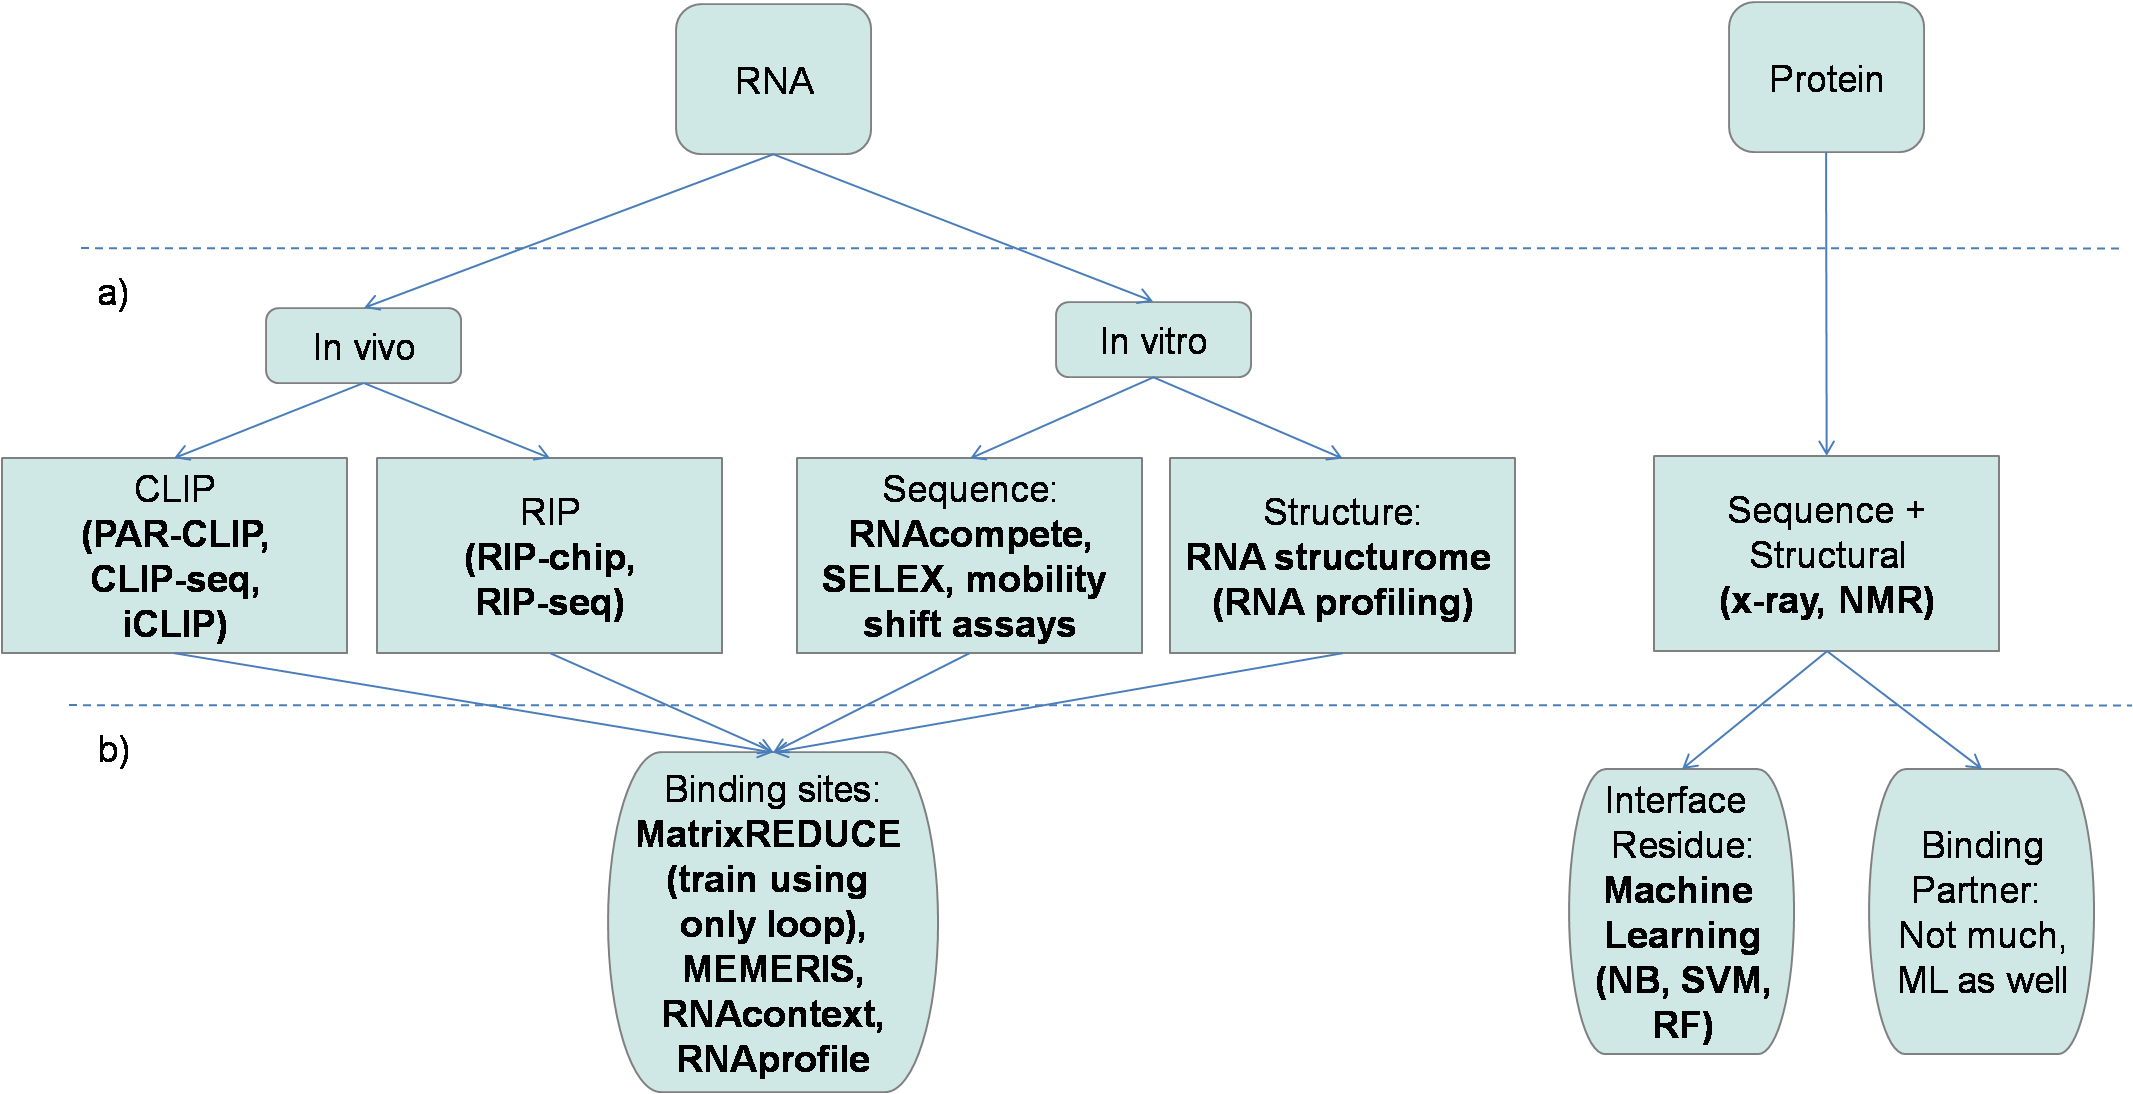
\includegraphics[width = \textwidth]{overview}
    \caption[Overview of RNA-protein interaction research]{\label{fig21} Overview of RNA-protein interaction research. a) experimental methods for RNA (both in vivo and in vitro) and protein binding sites detection. b) computational methods (in vitro RNA binding site is not of interest) }
  \end{center}
\end{figure}

Figure~\ref{fig21} is basically drawn with guidance of Peter Stadler's recent review paper \cite{Stadler2012}. The paper discussed both RNA-RNA and RNA-protein interactions. And both experimental and computational methods are reviewed. It also provides pointers to promising databases. Besides, I am very happy that, the "RNA-protein" and "database" sections of this paper are very similar to the literature review part of my RPE report, which shows my work is on the right track.



\subsection{Computational Methods}
For RNA-protein interactions, this review paper summarized that previous studies have shown that sequence-specific RBPs either recognize and bind to unstructured single-stranded RNA \cite{Ellis2007} or require at least some of their mRNA binding sites to be unpaired \cite{Li01062010}. Based on this point, several representative computational methods, RNAcontext, MEMERIS, Vienna+P and a work from Morris group are introduced. Besides, HuR protein is mentioned as a "model" to assess the binding sites accessibility since HuR binds to unpaired U-rich motifs in 3'UTR. 

Peter Stadler's recent review paper covers a wide range of this field and provides a very good guideline for my research. Besides of the works mentioned in his review, there are several other studies which are very relevant to my project.

Particularly, in a study \cite{Li01062010} from Morris group at UToronto, the accessibility of a target site or region on mRNA is calculated as the probability that the site or region is unpaired. \href{http://www.tbi.univie.ac.at/~ivo/RNA/RNAplfold.html}{RNAplfold} \cite{Bernhart01032006}, as minimum free energy (MFE) folding algorithm from Vienna package \cite{Bernhart2008} is used to estimate such probability. MFE folding algorithm predicts the secondary structure that minimizes the overall free energy of a RNA in thermodynamic equilibrium. In another word, such algorithm predicts the most stable structure. By taking accessibility into consideration, the accuracy of predicting RBP bindings has been significantly improved on benchmarked data \cite{Hogan2008}.

There is one recent paper uses a set of structural discovery algorithms followed by SVM training \cite{Xiaowei2012}. The authors trained a novel classification model (CisRNA-SVM) on a set of known structured cis-regulatory elements from 3'UTRs. Their data is selected from TargetScan. The interesting part is that the four programs chosen for the training process are RNAalifold, LocARNA, Foldalign and Cove. They represented four different categories of folding strategies: align-then-fold, fold-then-align, simultaneous fold-and-align and covariance-based methods.

There are also several recent papers \cite{Tomasz2012} which focus on protein side and its computational methods (mainly machine learning). Since this is not my focus and my RPE report shares large overlaps with these papers, no further descriptions here.



\subsection{Experimental datasets}
Besides of the computational methods, experimental datasets are also of great importance to my study. As shown in Figure~\ref{fig21}, from RNA side, there are in vivo experimental techniques RIP and CLIP, and in vitro techniques like SELEX and RNA profiling; from protein side, there are mostly structural techniques like x-ray and NMR. Here in this project, I will primarily focus on in vivo techniques for mRNA, mainly RIP and CLIP.



\subsubsection{RIP}
RIP is the conventional method for studying RNA-protein interactions. One benchmarked dataset that has been used in many computational papers is generated from Hogan \emph{et al.} \cite{Hogan2008}. It contains Yeast RIP-chip (RNA-binding protein immunoprecipitation coupled to reverse transcription and a microarray) data of 12,000 pairs of RBP-RNA interactions. It serves as the proof-of-principle data set for several previous studies \cite{Muppirala22192482, Li01062010}.

Lange \emph{et al.} have recently published a paper on predicting secondary structure and accessibility in mRNAs \cite{Lange28022012}. The paper provides two benchmarked datasets for secondary structures of mRNA functional elements: 2,500 structured cis-regulatory elements in 95 Rfam families, and 3,196 \emph{in vivo} Saccharomyces cervisiae mRNAs with secondary structure available.



\subsubsection{CLIP}
The recent cutting-edge technology for RNA-protein interactions is CLIP, i.e. high-throughput (UV) cross-linking immunoprecipitation technique. There is a nice review paper on all kinds of high-throughput CLIP methods \cite{Julian2012}. It also introduced downstream procedures to identify binding sites from sequencing data of CLIP. There are two major databases \href{http://www.clipz.unibas.ch/}{CLIPZ} and \href{http://dorina.mdc-berlin.de/rbp_browser/dorina.html}{doRiNA} which collect CLIP data generated from several recent large scale experiments. Each data set from these two database contains transcriptome-wide binding site data for both RBPs and miRNAs. DoRiNA hosts 17 such CLIP sets for Human, Mouse, C.elegans. And CLIPZ hosts 999,350 CLIP-determined AGO protein binding sequences for the same species.

Especially for doRiNA database, it is based on the thought that the combinatorial action of RBPs and miRNAs on target mRNAs form a post-transcriptional regulatory code. The authors \cite{Anders01012012} provide this database that supports the quest for deciphering this code. The database is built based on Hafner's PAR-CLIP data, supplement with other CLIP datasets. They assign two quality scores based on the characteristics of the PAR-CLIP protocol: \# of conversions and entropy of reads.


Since CLIP data is really new and of large scale, it may be very useful for the future studies of Protein-binding RNAs. While, it has many different variants like HITS-CLIP (normal form of CLIP), PAR-CLIP, iCLIP etc., and they are sometimes confusing to researchers in this field. So several representative papers are reviewed here as a comparison of different CLIP techniques. 

\paragraph{CLIP vs PAR-CLIP}
In this paper, the authors found only small differences in accuracies of these methods in identifying binding sites of HuR \cite{Shivendra2011}. To determine whether differences between protocols are reflected in the set of identified target sites, they started from PAR-CLIP and individually modified the two steps that are most likely to bias the identification of binding sites: cross-linking and RNase digestion.

\paragraph{CLIP vs PAR-CLIP vs iCLIP} 
The authors \cite{Chaolin2012} found that reverse transcriptase used in CLIP frequently skips the crosslinked amino-acid-RNA adduct, resulting in a nucleotide deletion, which is more precise of mapping protein-RNA interactions than currently available PAR-CLIP and iCLIP. The used Nova and Argonaut (Ago) HITS-CLIP data. Especially, the cross-linking induced mutation frequency in standard CLIP is lower than that observed from PAR-CLIP, but more meaningful comparisons have to consider signal-to-noise, which is \~15–50 fold for CIMS analysis (\~8–20\% crosslinking mutation rate vs. \~0.4–0.5\% background deletion rate due to sequencing or alignment errors), and 4–5 fold in PAR-CLIP (50–80\% cross-linking induced T–C transition vs. 10–20\% spontaneous transitions).

\paragraph{iPAR-CLIP}
In vivo PAR-CLIP (iPAR-CLIP) is introduced and performed in this paper \cite{Anna-Carina2011}. They use KH domain-containing RBP GLD-1 protein which is known to recognize a relatively well-defined primary sequence motif. Note that, according to the paper, Lebedeva2011 and Mukherjee2011 datasets (collected in doRiNA as well) are NOT in vivo.



\subsubsection{ENCODE}
In the recent published ENCODE project \cite{ENCODE2012}, There is a \href{http://genome.ucsc.edu/cgi-bin/hgTrackUi?db=hg19&g=wgEncodeRbpSuper}{RIP dataset} for several human RNA-binding proteins, but not been focused in ENCODE papers. 

The tracks in this supertrack contain two forms of information: genes whose transcripts were bound by the given RBP (such as \textbf{SUNY RIP GeneSt}) and approximate location of the RBP binding site in the mRNA sequence (such \textbf{SUNY RIP Tiling} and \textbf{SUNY RIP-seq}). An overview of the data is shown in Table~\ref{ENCODErip}

\begin{table}[ht]
  \begin{center}
    \begin{tabular}{|l||l|l||l|l|}
      \hline
      &\multicolumn{2}{l|}{RIP Tiling}&\multicolumn{2}{l|}{RIP-seq}\\
      \cline{2-5}
       &GM12878&K562&GM12878&K562\\
      \hline\hline
      ELAVL1&Y&Y&Y&Y\\
      PABPC1&Y&Y&Y&Y\\
      Negative Control&Y&Y&&\\
      Input(Total)&Y&Y&&\\
      \hline
    \end{tabular}
    \caption{
      \label{ENCODErip}
      The ENCODE datasets for RBP binding sites of \textit{Human}.}
  \end{center}
\end{table}

\FloatBarrier

And the files are mainly encoded in broadPeak formats. This format is used to provide called regions of signal enrichment based on pooled, normalized (interpreted) data. It is a BED 6+3 format. So besides of normal BED 6 format which has 6 columns to denote: chrom, chromStart, chromEnd, name, score, and strand, the broadPeak format has 3 additional columns: signalValue, pValue and qValue, which are measurements of enrichment for the region.

All the three tier 1 cell lines of ENCODE project are included:

\textbf{\textit{GM12878}} is a lymphoblastoid cell line produced from the blood of a female donor with northern and western European ancestry by EBV transformation. It was one of the original HapMap cell lines and has been selected by the International HapMap Project for deep sequencing using the Solexa/Illumina platform. This cell line has a relatively normal karyotype and grows well. Choice of this cell line offers potential synergy with the International HapMap Project and genetic variation studies. It represents the mesoderm cell lineage. Cells will be obtained from the Coriell Institute for Medical Research [coriell.org] (Catalog ID GM12878).

\textbf{\textit{K562}} is an immortalized cell line produced from a female patient with chronic myelogenous leukemia (CML). It is a widely used model for cell biology, biochemistry, and erythropoiesis. It grows well, is transfectable, and represents the mesoderm linage. Cells will be obtained from the America Type Culture Collection (ATCC) [atcc.org] (ATCC Number CCL-243).

\textbf{\textit{H1 human embryonic stem cells}} will be obtained from Cellular Dynamics International [cellulardynamics.com].




\section{The proposed study}
In this project, we propose to assess the secondary structural features of \emph{in vivo} protein binding sites on mRNA transcripts. mRNA sequences have the remarkable ability to form structures which define the functional roles they play in the cell. Proteins, in turn, are known to recognize and bind to certain RNA transcripts with specific structures in a sequence-specific or unspecific way. Currently, there already exist a number of known protein binding sites in mRNA sequences. While, there are only a few computational methods have considered the structural features of these binding sites previously\cite{Li01062010, Pancaldi01042011}, and they all assume that the RNA transcript folds into its thermodynamically most stable structure. 

We know, however, that this assumption generally does not hold \emph{in vivo}. Previous research has shown that the optimized thermodynamic structure does not necessarily correspond to the structure that is functional in the cell, especially for molecules such as pre-mRNAs and long mRNAs \cite{Morgan1996}. The reasons may be the effect of co-transcriptional folding \cite{Meyer15298702} (when the mRNA molecule is being transcribed, it folds at the same time; during this process, the mRNA forms a series of structures which are not the same as the thermodynamic structure) and the influence of other molecules binding the mRNA molecule.

We therefore propose to employ most widely used comparative methods instead to detect evolutionarily conserved RNA structures. These methods include Pfold \cite{Knudsen01072003}, RNAalifold \cite{Bernhart2008}, and RNA-Decoder \cite{Pedersen01012004}, which do not make the above thermodynamic assumption. Comparative methods in general tend to outperform thermodynamic methods in terms of prediction accuracy \cite{Meyer01112007}. They make use of the evolutionary information from homologous RNA sequences by assuming that homologous RNAs which have similar functions may also have similar structures for carrying out their biological functions \emph{in vivo}. Besides, as a key part of the project, the data set for mRNA-protein interactions is of crucial importance. Recently, several large scale experiments have identified a number of protein-RNA interactions, which makes it possible to systematically study the features of protein binding sites in RNA sequences.

The work has the potential to:
\begin{enumerate} 
\item contribute a systematic study of mRNA-protein interactions,  
\item increase the prediction accuracy of protein binding sites and,  
\item detect new types of RNA-protein interactions.
\end{enumerate}









\chapter{Results}
In this project, we assess the accessibility of mRNAs on both motif-wise and base-wise. Here \textbf{motif-wise accessibility} means that we compute the accessibility values for each protein binding motif by taking all the bases in the motif into consideration. And \textbf{base-wise accessibility} is based on comparisons of accessibilities between all binding motif positions and all UTR positions at individual base/position level. A motif is a sub-string that contains several consecutive bases on the transcript, normally on 3'UTR region. In general, we want to see if there is any difference of accessibilities between motif region and the background whole UTR region on each transcript. 

Here, we apply three comparative methods:
\begin{itemize}
\item \href{http://www.daimi.au.dk/~compbio/pfold/}{Pfold}
\item \href{rna.tbi.univie.ac.at/cgi-bin/RNAalifold.cgi}{RNAalifold}
\item \href{http://www.ebi.ac.uk/~meyer/rnadecoder}{RNA-Decoder}
\end{itemize} 

And we use two measurements to define the \textbf{accessibility}: 
\begin{description}
\item[A.] the rate of the base-pairing cases in binding sites according to the consensus structures ("fold" mode);
\item[B.] the base-pairing probability across binding sites ("scan" mode).
\end{description}
So for each of the three programs, we calculate the values of (A) and (B) for every RNA-binding protein which has binding sites information available in our dataset.
 
Besides, when calculating base paring probabilities (B) and consensus structures (A), they are calculated according to different regions: N (non-structured region), P (paired region), L (loop/bulge region) for both binding sites and (3'UTR) background sites. In below, I will use NPL to denote such classification.




% Sections are a sub-unit
\section{RNA-binding proteins and binding sites}
In this study, RNA-binding proteins and binding sites are derived from \cite{Li01062010}. The data is originally generated by RNP immunoprecipitation-microarray (RIP-chip) experiment. All together, it comprises 18 previously defined RBPs that bind to 3'UTR region of Yeast, Human and Fly mRNA sequences, and has consensus binding sequences (motif) available (Table~\ref{RBPs}). We map back these binding sequences to the corresponding transcripts (and alignments) using a sliding-window based approach.

We download from UCSC Genome Browser \cite{Fujita18102010} the genomes and corresponding multiple genomic sequence alignments for Yeast, Human and Fly species. In order to compare with the work in \cite{Li01062010}, we choose the same versions as in that paper, namely Yeast (sacCer2, i.e. SGD1.01), Human (hg18) and Fly (dm3, i.e. BDGP Release 5). We also downloaded the annotation for each genome from the Ensembl database \cite{Flicek01012011}. We use a tool, mafsInRegion from UCSC to fetch all of the mRNA transcripts (whole transcript and the three prime untranslated region (3'UTR)) from each genomes' multiple species alignments. We then utilize a widely used perl library Bioperl \cite{Stajich01102002} (version 1.006001) to convert the raw UCSC alignments from maf format to different formats as required by the different programs.


\subsection{Overview of RBPs}
\FloatBarrier

For each of these proteins, the primary sources of its binding information are NCBI, InterPro and UniProt. Besides, for the binding type, the information is directly got from these databases (very rare), or from PDB and GO database (structure from PDB; ss or ds term associated in GO), or from individual sources including species’ database, like SGD (Saccharomyces Genome Database) or other protein database, like SMART or Pfam, or individual papers. The source of the binding type is annotated in the parentheses in the table below.

\iffalse
\begin{center}
  \begin{longtable}{|l|l|l|l|l|}
    \caption{\label{RBPs} Overview of Yeast RBPs}\\
   
   
   
   
    \hline \multicolumn{1}{|c|}{\textbf{RBPs}} &
    \multicolumn{1}{c|}{\textbf{Motif}} &
    \multicolumn{1}{c|}{\textbf{Binding type}} &
    \multicolumn{1}{c|}{\textbf{Database ID}} &
    \multicolumn{1}{c|}{\textbf{Database Info}} \\ \hline
    \endfirsthead

    \multicolumn{5}{c}%
    {{\bfseries \tablename\ \thetable{} -- continued from previous page}} \\
    \hline \multicolumn{1}{|c|}{\textbf{RBPs}} &
    \multicolumn{1}{c|}{\textbf{Motif}} &
    \multicolumn{1}{c|}{\textbf{Binding type}} &
    \multicolumn{1}{c|}{\textbf{PDB ID}} &
    \multicolumn{1}{c|}{\textbf{PDB Info}} \\ \hline
    \endhead

    \hline \multicolumn{5}{|r|}{{Continued on next page}} \\ \hline
    \endfoot

    \hline \hline
    \endlastfoot
  
   
   
    Msl5 & UACUAAC & & UniProt:Q12186 & pre-mRNA branch point binding\\
    Puf4 & UGUAHMNUA & single & PDB: 3BX3 3BWT 3BX2 4DZS &  \\
    Puf3 & CNUGUAHAUA & single & PDB: 3K49 3K4E&  \\
    Khd1 & CNNCNN &  & &  \\
    Nab2 & DRARAMGMD &  &  PDB: 2JPS 2V75 & form complex with Gfd1 \\
    Yll032c & AAUACCY &  & &  \\
    Vts1 & CNGG &  &  PDB: 2D3D 2FE9 2B6G 2F8K 2ES6 2ESE &  bind an RNA hairpin termed the Smaug recognition element (SRE) \\
    Pub1 & HUUUUUUHW &  & PDB: 2LA4 3MD1 3MD3 &  poly(A)+ mRNA binding \\
    Puf2 & UAAUAAW &  & &  \\
    Puf5 & WUUGUAWUWU &  & & Homolog of Fly Pumilio\\
    Ssd1 & AKUCAUUCCUU &  & UniProt:P24276 & RNR ribonuclease family \\
    PAB1 & WUAUAUAW &  & PDB:1IFW & contains PABC domain which is poly(A)- binding \\
    Nsr1 & GGGWAACGGW &  & &  \\
    Nrd1 & UUCUUGUW &  & PDB:3CLJ & By recruiting it to RNA Pol II, Nrd1 could cooperate with Nab3 and Sen1 to terminate small nucleolar RNAs and other short RNAs. \\  
\end{longtable}
\end{center}

\begin{table}[ht]
  \begin{center}
    \begin{tabular}{|l||l|l||l|l|}
      \hline \multicolumn{1}{|c|}{\textbf{RBPs}} &
    \multicolumn{1}{c|}{\textbf{Motif}} &
    \multicolumn{1}{c|}{\textbf{Binding type}} &
    \multicolumn{1}{c|}{\textbf{Database ID}} &
    \multicolumn{1}{c|}{\textbf{Database Info}} \\ \hline
    \hline \hline
   
    Msl5 & UACUAAC & & UniProt:Q12186 & pre-mRNA branch point binding\\
    Puf4 & UGUAHMNUA & single & PDB: 3BX3 3BWT 3BX2 4DZS &  \\
    Puf3 & CNUGUAHAUA & single & PDB: 3K49 3K4E&  \\
    Khd1 & CNNCNN &  & &  \\
    Nab2 & DRARAMGMD &  &  PDB: 2JPS 2V75 & form complex with Gfd1 \\
    Yll032c & AAUACCY &  & &  \\
    Vts1 & CNGG &  &  PDB: 2D3D 2FE9 2B6G 2F8K 2ES6 2ESE &  bind an RNA hairpin termed the Smaug recognition element (SRE) \\
    Pub1 & HUUUUUUHW &  & PDB: 2LA4 3MD1 3MD3 &  poly(A)+ mRNA binding \\
    Puf2 & UAAUAAW &  & &  \\
    Puf5 & WUUGUAWUWU &  & & Homolog of Fly Pumilio\\
    Ssd1 & AKUCAUUCCUU &  & UniProt:P24276 & RNR ribonuclease family \\
    PAB1 & WUAUAUAW &  & PDB:1IFW & contains PABC domain which is poly(A)- binding \\
    Nsr1 & GGGWAACGGW &  & &  \\
    Nrd1 & UUCUUGUW &  & PDB:3CLJ & By recruiting it to RNA Pol II, Nrd1 could cooperate with Nab3 and Sen1 to terminate small nucleolar RNAs and other short RNAs. \\  

      \hline
    \end{tabular}
    \caption{
      \label{RBPs}
      Overview of Yeast RBPs.}
  \end{center}
\end{table}
\fi


\begin{longtable}{*{1}{p{30pt}}|*{1}{p{85pt}}|*{1}{p{45pt}}|*{1}{p{65pt}}|*{1}{p{120pt}}}%{lllll} %{{}{}{}{}{p{48pt}}}
\caption{\label{RBPs} Overview of Yeast RBPs.}
    \\
    \hline%\toprule
    \hline
    \textbf{RBPs}&\textbf{Motif}&\textbf{Binding type}&\textbf{Database ID}&\textbf{Remark}\\
    \hline\hline%\midrule
    Msl5 & UACUAAC & single (inferred from its KH domain) & PDB: 3FMA & pre-mRNA branch point binding; AU-rich elements binding (see AREsite); cooperatively recognize a tetra-loop structure \cite{GarciaMayoral2007485}\\\hline
    Puf4 & UGUAHMNUA & single (PDB) & PDB: 3BX3 3BWT 3BX2 4DZS & Puf3, Puf4 and Puf5 in Yeast, and Pum1 in humans, are known to bind \href{http://www.mun.ca/biology/scarr/Tetranucleotide_Hypothesis.html}{UGUR tetranucleotide motif} \cite{Leibovich13032012}\\\hline
    Puf3 & CNUGUAHAUA & single (PDB) & PDB: 3K49 3K4E & PUF protein family \\\hline
    Khd1 & CNNCNN & single (inferred from its KH domain) & InterPro: P38199 & aka HEK2, YBL032W; AU-rich elements binding (see AREsite)  \\\hline
    Nab2 & DRARAMGMD &  &  PDB: 2JPS 2V75 2LHN 3LCN 4H1K & form complex with Gfd1; poly(A) RNA binding  \\\hline
    Yll032c & AAUACCY &  single (inferred from its KH domain) & &  Protein of unknown function that may interact with ribosomes; KH domain contained \\\hline
    Vts1 & CNGG & single (NCBI, GO) &  PDB: 2D3D 2FE9 2B6G 2F8K 2ES6 2ESE &  bind an RNA hairpin termed the Smaug recognition element (SRE); flap-structured DNA and RNA binding (GO) \\\hline
    Pub1 & HUUUUUUHW & single (InterPro) & PDB: 2LA4 3MD1 3MD3 &  poly(A)+ mRNA binding; RRM domain (single-stranded RNA binding) contained \\\hline
    Puf2 & UAAUAAW & single (inferred from other PUF proteins) & UniProt: Q12221 & Member of the PUF protein family, like Puf4 etc., Pumilio homology domain contained; RRM domain contained \\\hline
    Puf5 & WUUGUAWUWU &  single (inferred from other PUF proteins) & UniProt: P39016 & see Puf4, Pumilio domain contained; \\\hline
    Ssd1 & AKUCAUUCCUU & single (PDB Homolog) & UniProt: P24276; PDB: 2VNU 2WP8 4IFD (homolog according to PROSITE and SGD) & RNR ribonuclease family \\\hline
    PAB1 & WUAUAUAW & single (inferred from its RRM domain) & PDB: 1IFW & contains PABC domain which is poly(A) binding; RRM domain contained \\\hline
    Nsr1 & GGGWAACGGW & single (inferred from its RRM domain) & UniProt: P27476 & RRM domain contained; nucleolar protein that binds nuclear localization sequences; required for pre-rRNA processing; single-stranded DNA binding \\\hline
    Nrd1 & UUCUUGUW & single (inferred from its RRM domain) & PDB: 2LO6 3CLJ & By recruiting it to RNA Pol II, Nrd1 could cooperate with Nab3 and Sen1 to terminate small nucleolar RNAs and other short RNAs; 3'-end processing of mRNA, snoRNA, snRNA and tRNA; RRM domain contained \\\hline
    Pum1 & UGUAHAUA & single (inferred from other PUF proteins) & PDB: 1m8z (homolog) & Pumilio homolog; PUF protein family %\\\hline
    \\   \hline\hline%\bottomrule
\end{longtable}

\FloatBarrier
Note that, for those RBPs which have different binding motifs, combine by picking the most general one (eg. for CNGG and CNGGN, pick CNGG).



\subsubsection{Detailed description of RBPs}
\paragraph{Msl5}
\begin{enumerate}
\item \textit{Species} Yeast
\item \textit{Function} nuclear mRNA splicing, via spliceosome
\item \textit{Domain} KH, 2ZnF\_C2H2
\item \textit{Description} Component of the commitment complex, which defines the first step in the splicing pathway; essential protein that interacts with Mud2p and Prp40p, forming a bridge between the intron ends; also involved in nuclear retention of pre-mRNA.
\end{enumerate}

\iffalse
\subparagraph{Species}
Yeast
\subparagraph{Function}
nuclear mRNA splicing, via spliceosome
\subparagraph{Domain}
KH, 2ZnF\_C2H2
\subparagraph{Description}
Component of the commitment complex, which defines the first step in the splicing pathway; essential protein that interacts with Mud2p and Prp40p, forming a bridge between the intron ends; also involved in nuclear retention of pre-mRNA.
\fi


\paragraph{Puf4}
\begin{enumerate}
\item \textit{Species} Yeast
\item \textit{Function} Loss of chromatin silencing during replicative cell aging, mRNA catabolic process, nuclear-transcribed mRNA catabolic process, deadenylation-dependent decay, protein localization.
\item \textit{Domain} 8Pumilio repeat
\item \textit{Description} Member of the PUF protein family, which is defined by the presence of Pumilio homology domains that confer RNA binding activity; preferentially binds mRNAs encoding nucleolar ribosomal RNA-processing factors.
\end{enumerate}


\paragraph{Puf3}
\begin{enumerate}
\item \textit{Species} Yeast
\item \textit{Function} aerobic respiration, intracellular mRNA localization, mitochondrion localization, mitochondrion organization, nuclear-transcribed mRNA catabolic process, nuclear-transcribed mRNA catabolic process, deadenylation-dependent decay.
\item \textit{Domain} 8Pumilio repeat
\item \textit{Description} Protein of the mitochondrial outer surface, links the Arp2/3 complex with the mitochore during anterograde mitochondrial movement; also binds to and promotes degradation of mRNAs for select nuclear-encoded mitochondrial proteins.
\end{enumerate}


\paragraph{Khd1}
\begin{enumerate}
\item \textit{Species} Yeast
\item \textit{Function} Cytoplasm, nuclear chromosome, telomeric region.
\item \textit{Domain} 3KH
\item \textit{Description} RNA binding protein involved in the asymmetric localization of ASH1 mRNA; represses translation of ASH1 mRNA, an effect reversed by Yck1p-dependent phosphoryation; regulates telomere position effect and length; similarity to hnRNP-K.
\end{enumerate}


\paragraph{Nab2}
\begin{enumerate}
\item \textit{Species} Yeast
\item \textit{Function} mRNA polyadenylation, poly(A+) mRNA export from nucleus, regulation of mRNA stability.
\item \textit{Domain} coiled coil
\item \textit{Description} Nuclear polyadenylated RNA-binding protein required for nuclear mRNA export and poly(A) tail length control; binds nuclear pore protein Mlp1p; autoregulates mRNA levels; related to human hnRNPs; nuclear localization sequence binds Kap104p.
\end{enumerate}


\paragraph{Yll032c}
\begin{enumerate}
\item \textit{Species} Yeast
\item \textit{Domain} KH
\item \textit{Description} Protein of unknown function that may interact with ribosomes, based on co-purification experiments; green fluorescent protein (GFP)-fusion protein localizes to the cytoplasm; YLL032C is not an essential gene. Not use.
\end{enumerate}


\paragraph{Vts1}
\begin{enumerate}
\item \textit{Species} Yeast
\item \textit{Function} Nuclear-transcribed mRNA catabolic process, Nuclear-transcribed mRNA poly(A) tail shortening.
\item \textit{Domain} Vts1
\item \textit{Description} Post-transcriptional gene regulator, RNA-binding protein containing a SAM domain; shows genetic interactions with Vti1p, which is a v-SNARE involved in cis-Golgi membrane traffic.
\end{enumerate}


\paragraph{Pub1}
\begin{enumerate}
\item \textit{Species} Yeast
\item \textit{Function} Nuclear-transcribed mRNA catabolic process, nonsense-mediated decay, regulation of mRNA stability, stress granule assembly.
\item \textit{Domain} 3RRM
\item \textit{Description} Poly (A)+ RNA-binding protein, abundant mRNP-component protein that binds mRNA and is required for stability of many mRNAs; component of glucose deprivation induced stress granules, involved in P-body-dependent granule assembly.
\end{enumerate}


\paragraph{Puf2}
\begin{enumerate}
\item \textit{Species} Yeast
\item \textit{Function} Nuclear-transcribed mRNA catabolic process, deadenylation-dependent decay.
\item \textit{Domain} 6Pumilio, RRM
\item \textit{Description} Member of the PUF protein family, which is defined by the presence of Pumilio homology domains that confer RNA binding activity; preferentially binds mRNAs encoding membrane-associated proteins.
\end{enumerate}


\paragraph{Puf5}
\begin{enumerate}
\item \textit{Species} Yeast
\item \textit{Function} Cell wall organization, loss of chromatin silencing during replicative cell agin, nuclear-transcribed mRNA catabolic process, deadenylation-dependent decay, protein localization, re-entry into mitotic cell cycle after pheromone arrest, replicative cell aging.
\item \textit{Domain} 8Pumilio repeat
\item \textit{Description} Member of the Puf family of RNA-binding proteins; binds to mRNAs encoding chromatin modifiers and spindle pole body components; involved in longevity, maintenance of cell wall integrity, and sensitivity to and recovery from pheromone arrest
\end{enumerate}


\paragraph{Ssd1}
\begin{enumerate}
\item \textit{Species} Yeast
\item \textit{Function} RNA binding, cell wall organization, chronological cell aging, replicative cell aging, response to drug.
\item \textit{Domain} Coiled coil
\item \textit{Description} Protein with a role in maintenance of cellular integrity, interacts with components of the TOR pathway; ssd1 mutant of a clinical S. cerevisiae strain displays elevated virulence.
\end{enumerate}


\paragraph{PAB1}
\begin{enumerate}
\item \textit{Species} Yeast
\item \textit{Function} Regulation of translational initiation.
\item \textit{Domain} 4RRM, PolyA
\item \textit{Description} Poly(A) binding protein, part of the 3'-end RNA-processing complex, mediates interactions between the 5' cap structure and the 3' mRNA poly(A) tail, involved in control of poly(A) tail length, interacts with translation factor eIF-4G.
\end{enumerate}


\paragraph{Nsr1}
\begin{enumerate}
\item \textit{Species} Yeast
\item \textit{Function} Ribosomal small subunit assembly, rRNA processing.
\item \textit{Domain} 2RRM, coiled coil
\item \textit{Description} Nucleolar protein that binds nuclear localization sequences, required for pre-rRNA processing and ribosome biogenesis.
\end{enumerate}


\paragraph{Nrd1}
\begin{enumerate}
\item \textit{Species} Yeast
\item \textit{Function} Termination of RNA polymerase II transcription, poly (A)-independent.
\item \textit{Domain} RPR, RRM
\item \textit{Description} RNA-binding protein that interacts with the C-terminal domain of the RNA polymerase II large subunit (Rpo21p), preferentially at phosphorylated Ser5; required for transcription termination and 3' end maturation of nonpolyadenylated RNAs.
\end{enumerate}


\paragraph{Pumilio}
\begin{enumerate}
\item \textit{Species} Fly
\item \textit{Function} mRNA 3'-UTR binding; protein binding; mRNA binding; translation repressor activity, nucleic acid binding.
\item \textit{Domain} 8Pumilio repeat, coiled coil
\item \textit{Description} The gene pumilio is referred to in FlyBase by the symbol Dmel\\pum (CG9755, FBgn0003165). The phenotypes of these alleles are annotated with 46 unique terms, many of which group under: organ system; embryonic abdomen; embryonic segment; anatomical structure; female germline cyst; nervous system; embryonic tagma; peripheral nervous system; germarium; embryonic neuron; multi-cell-component structure; cephalopharyngeal skeleton. It has 5 annotated transcripts and 5 annotated polypeptides.
\end{enumerate}


\paragraph{HuR}
\begin{enumerate}
\item \textit{Species} Human
\item \textit{Function} multicellular organismal development, mRNA stabilization.
\item \textit{Domain} 3RRM
\item \textit{Description} The protein encoded by this gene is a member of the ELAVL protein family. This encoded protein contains 3 RNA-binding domains and binds cis-acting AU-rich elements. It destabilizes mRNAs and thereby regulates gene expression.
\end{enumerate}


\paragraph{Pum1}
\begin{enumerate}
\item \textit{Species} Human
\item \textit{Function} Membrane organization, post-Golgi vesicle-mediated transport, regulation of translation.
\item \textit{Domain} Cytoplasm, cytosol
\item \textit{Description} A member of the PUF family, evolutionarily conserved RNA-binding proteins related to the Pumilio proteins of Drosophila and the fem-3 mRNA binding factor proteins of C. elegans. The encoded protein contains a sequence-specific RNA binding domain comprised of eight repeats and N- and C-terminal flanking regions, and serves as a translational regulator of specific mRNAs by binding to their 3' untranslated regions. The evolutionarily conserved function of the encoded protein in invertebrates and lower vertebrates suggests that the human protein may be involved in translational regulation of embryogenesis, and cell development and differentiation. Alternatively spliced transcript variants encoding different isoforms have been described. 
\end{enumerate}


\paragraph{PTB}
\begin{enumerate}
\item \textit{Species} Human
\item \textit{Function} RNA binding, Nucleotide binding, poly-pyrimidine tract binding, protein binding.
\item \textit{Domain} 4RRM
\item \textit{Description} This protein belongs to the subfamily of ubiquitously expressed heterogeneous nuclear ribonucleoproteins (hnRNPs). The hnRNPs are RNA-binding proteins and they complex with heterogeneous nuclear RNA (hnRNA). These proteins are associated with pre-mRNAs in the nucleus and appear to influence pre-mRNA processing and other aspects of mRNA metabolism and transport. While all of the hnRNPs are present in the nucleus, some seem to shuttle between the nucleus and the cytoplasm. The hnRNP proteins have distinct nucleic acid binding properties. The protein encoded by this gene has four repeats of quasi-RNA recognition motif (RRM) domains that bind RNAs. This protein binds to the intronic polypyrimidine tracts that requires pre-mRNA splicing and acts via the protein degradation ubiquitin-proteasome pathway. It may also promote the binding of U2 snRNP to pre-mRNAs. This protein is localized in the nucleoplasm and it is also detected in the perinucleolar structure. Alternatively spliced transcript variants encoding different isoforms have been described.
\end{enumerate}


%------------comment out by syang: Start----------------
\iffalse
\begin{table}[ht]
  \begin{center}
    \begin{tabular}{|l||l|l||l|l|}
      \hline
      &\multicolumn{2}{l|}{Conservation}&\multicolumn{2}{l|}{Gappiness}\\
      \cline{2-5}
       &UCSC&\textbf{Realigned}&UCSC&\textbf{Realigned}\\
      \hline\hline
      mean&0.566&\textbf{0.544}&0.245&\textbf{0.232}\\
      std&0.105&\textbf{0.115}&0.117&\textbf{0.116}\\
%      3rd Person&at him&\textbf{aige}&at them&\textbf{acu}\\
%       &at her&\textbf{aici}& & \\
      \hline
    \end{tabular}
    \caption{
      \label{RBPs}
      The alignment quality scores for the raw UCSC alignments and the realigned alignments of \textit{Yeast}.}
  \end{center}
\end{table}
%------------comment out by syang: End----------------
\fi


%Since there are too many of RBPs and the input alignments need to be further realigned, plots are not listed here. But the raw data of "scan" and "fold" results are saved, in case of further comparison between original alignments results and realigned results.




\subsection{Base-wise accessibility}
As described at the beginning of this chapter, the study of \textbf{base-wise accessibility} here is based on comparisons between all binding motif positions and all UTR positions at single base/position level. We would like to detect if there is any difference between the accessibilities at motif region and background region. 

And as a pilot study, here we focus on the Pumilio protein of Fly species. We first look at only those transcripts with single UTR (around 7000 such transcripts). So for each of the three programs Pfold, RNAalifold and RNA-Decoder, we run it in both "scan" and "fold" modes respectively with NPL classification, as described at the beginning of this chapter.

\subsubsection{"Scan" mode}
\textbf{\textit{Definition}}: A binding motif is a sub-string on the UTR sequence, which matches a particular protein binding consensus profile as shown in Table ~\ref{RBPs}. A binding site is a base within a binding motif. "Scan" mode is to assign a pairing probability to each single base. And the $base \, wise\, accessibility = 1 - P(Pairing)$.

As we can see from Figure\ref{fig2} and \ref{fig3}, for PPfold and RNAalifold, the averaged base-wise pairing probabilities at background paired regions (3'UTR, P) are higher than those at binding motif paired regions (binding sites, P). But for RNAdecoder\ref{fig1}, it is not the case. Besides at loop regions and non-structured regions (L and N), neither the averaged pairing probabilities of background nor of binding motif is consistently stronger than the other.

\FloatBarrier
\begin{figure}[!hbp]
  \begin{center}
%% psfrag: comment the following line if not using the psfrag package
%    \psfrag{pie makes me happy!}{$\pi$ makes me happy!}
%% includegraphics: comment the following if not using the graphicx package
    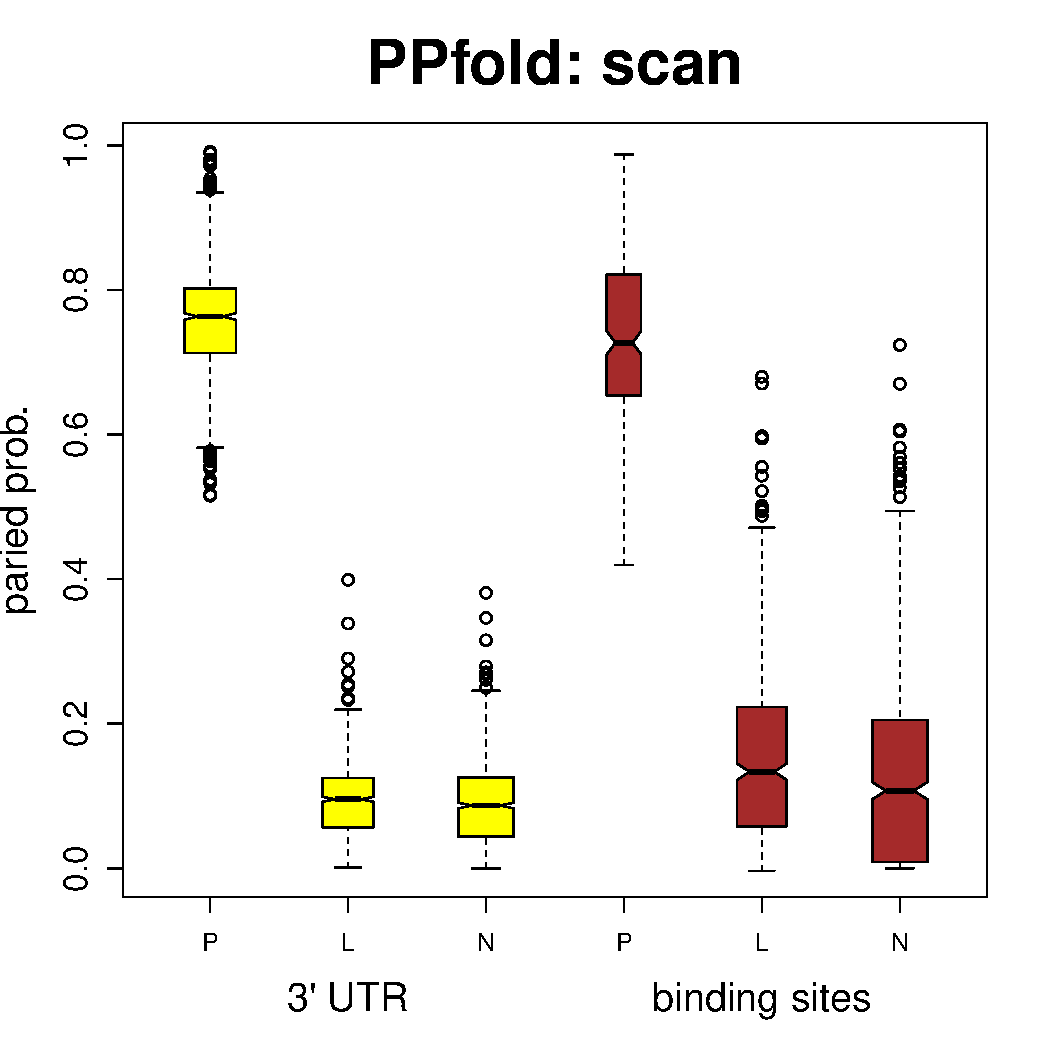
\includegraphics[width = 0.6\textwidth]{pfold_bp_npl_group}
    \caption[PPfold: Boxplot of base-pairing probabilities for protein binding sites and 3'UTR.]{\label{fig2} Boxplot of base-pairing probabilities for Pumilio binding sites positions and 3'UTR positions. The base-pairing probabilities are generated by PPfold for each alignment position. For each transcript, the probabilities of positions within binding sites region and those in background region (3'UTR) are averaged respectively, and then plotted for comparison.}
  \end{center}
\end{figure}

\begin{figure}[!hbp]
  \begin{center}
    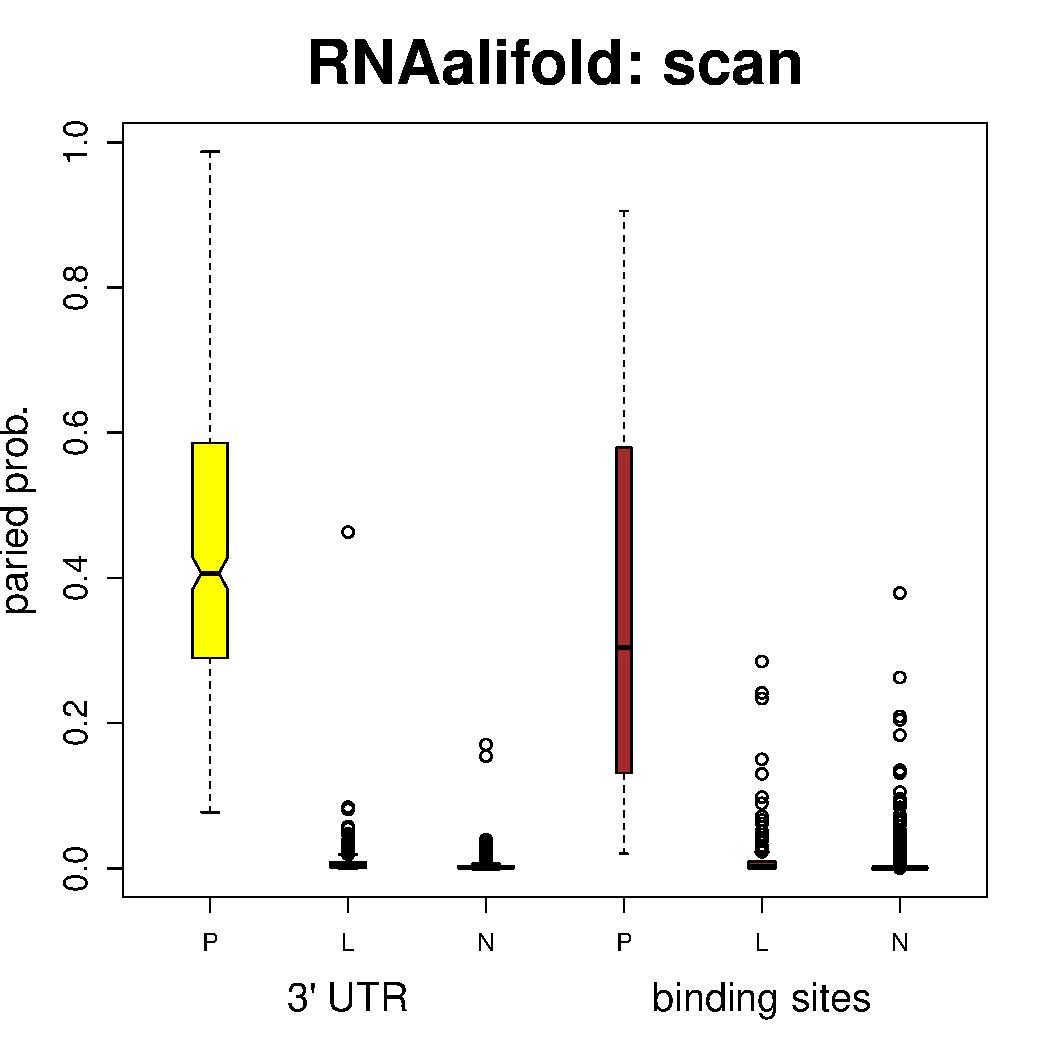
\includegraphics[width = 0.6\textwidth]{alifold_bp_npl_group}
    \caption[RNAalifold: Boxplot of base-pairing probabilities for protein binding sites and 3'UTR.]{\label{fig3} Boxplot of base-pairing probabilities for Pumilio binding sites positions and 3'UTR positions. The base-pairing probabilities are generated by RNAalifold for each alignment position. For each transcript, the probabilities of positions within binding sites region and those in background region (3'UTR) are averaged respectively, and then plotted for comparison.}
  \end{center}
\end{figure}

\begin{figure}[!hbp]
  \begin{center}
    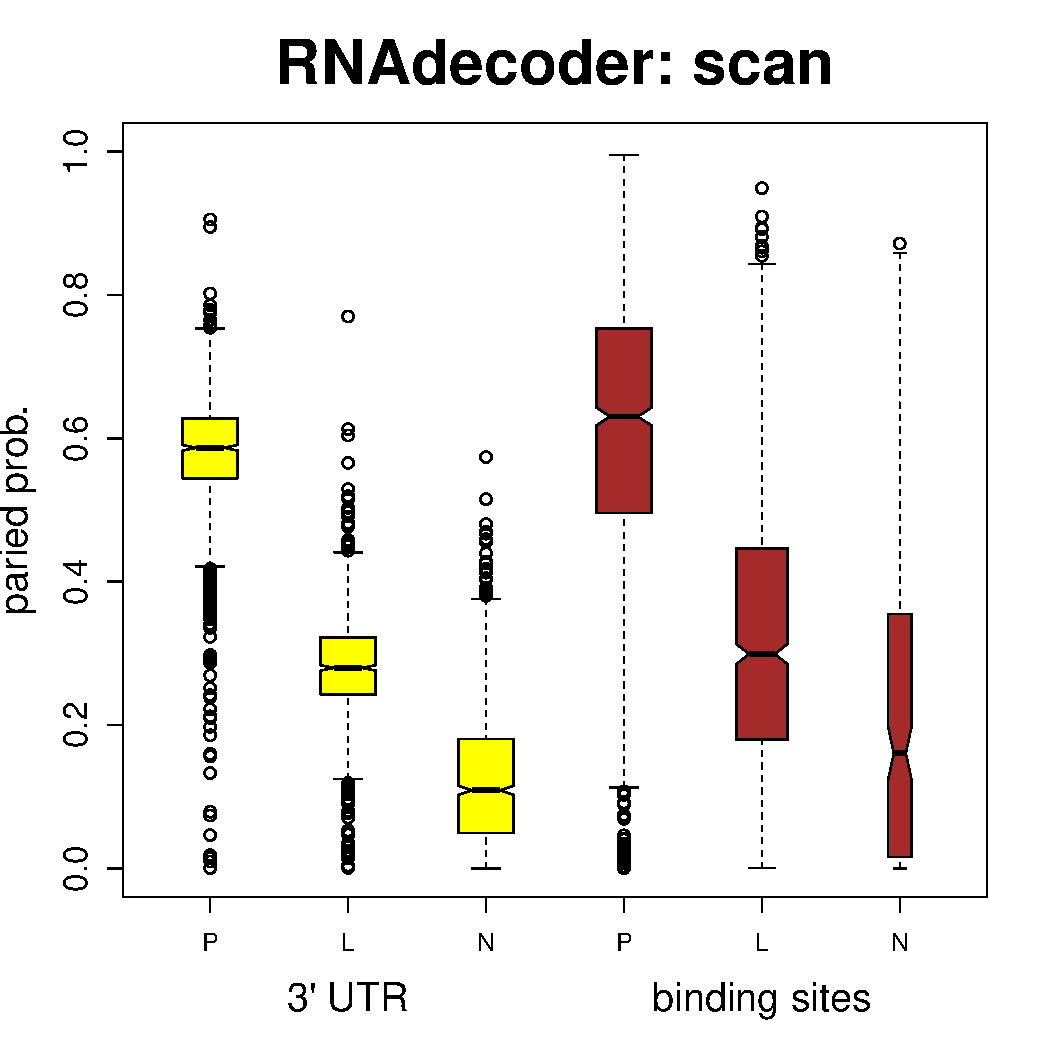
\includegraphics[width = 0.6\textwidth]{decoder_bp_npl_group}
    \caption[RNAdecoder: Boxplot of base-pairing probabilities for protein binding sites and 3'UTR.]{\label{fig1} Boxplot of base-pairing probabilities for Pumilio binding sites positions and 3'UTR positions. The base-pairing probabilities are generated by RNAdecoder for each alignment position. For each transcript, the probabilities of positions within binding sites region and those in background region (3'UTR) are averaged respectively, and then plotted for comparison.}
  \end{center}
\end{figure}
\FloatBarrier




\subsubsection{"Fold" mode}
\textbf{\textit{Definition}}: "Fold" mode is the labeling process, it is aimed to assign a consensus label (one out of N,L,P) to a given base. Here the probability computed is the frequency of a label x $\epsilon$ \{N,L,P\}, P(x) = (count of sites labeled with x)/(count of the total sites). 


As we can see from Figure\ref{fig4}, \ref{fig5} and \ref{fig6}, different programs have obvious different strategies when predicting consensus structures. RNAdecoder tends to predict more base pairs (Figure\ref{fig4}); while RNAalifold tends to predict less base pairs (i.e. less structures) (Figure\ref{fig5}); PPfold is in between (Figure\ref{fig6}). In general, the background regions have relatively more base pairing rates (P) and loop rates (L) than binding sites regions and less non-structured rates (N), which is as expected. 

\FloatBarrier
\begin{figure}[!hbp]
  \begin{center}
    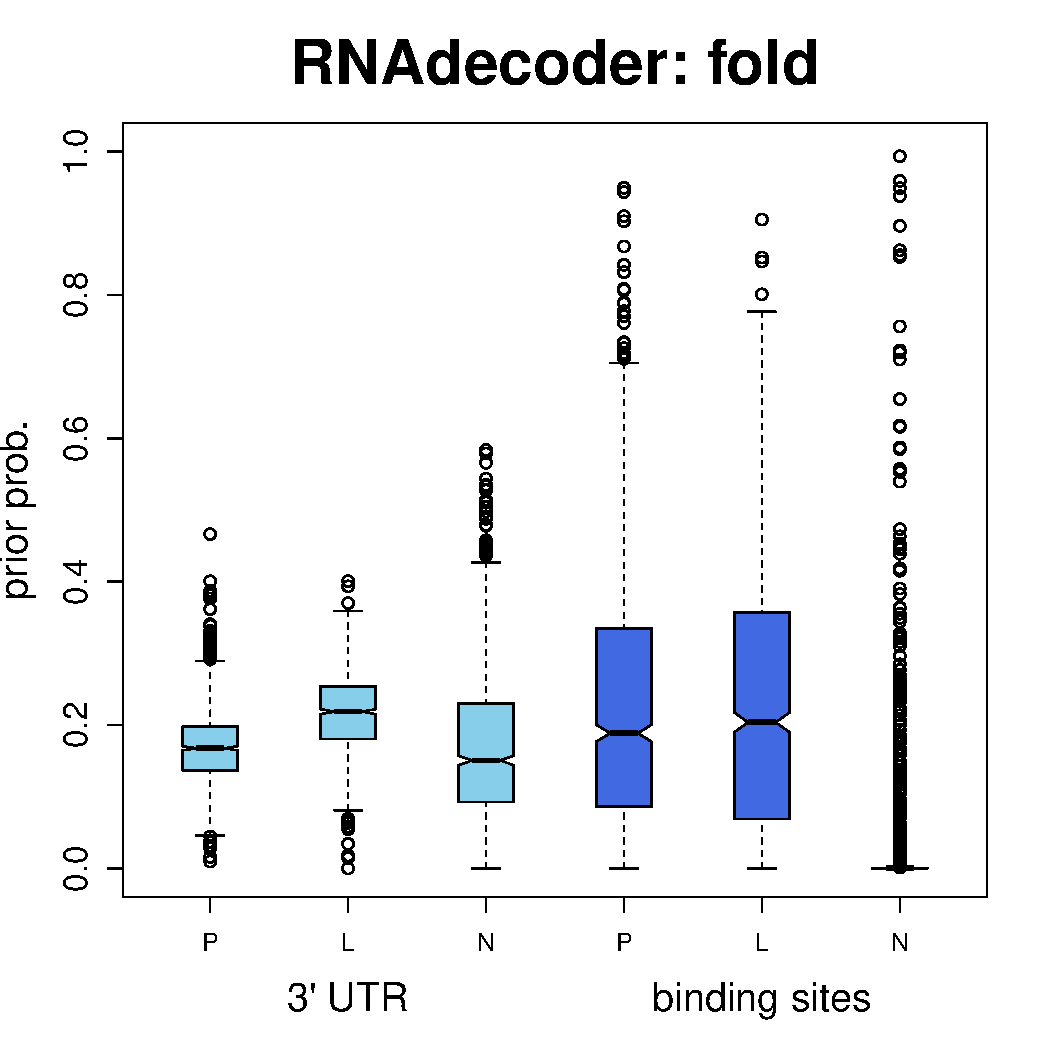
\includegraphics[width = 0.6\textwidth]{decoder_fd_npl_group}
    \caption[RNAdecoder: Boxplot of structural annotation probabilities for protein binding sites and 3'UTR.]{\label{fig4} Boxplot of structural annotation probabilities for Pumilio binding sites positions and 3'UTR positions. The structural annotation probabilities are generated by RNAdecoder for each alignment position. For each transcript, the probabilities of positions within binding sites region and those in background region (3'UTR) are averaged respectively, and then plotted for comparison.}
  \end{center}
\end{figure}

\begin{figure}[!hbp]
  \begin{center}
    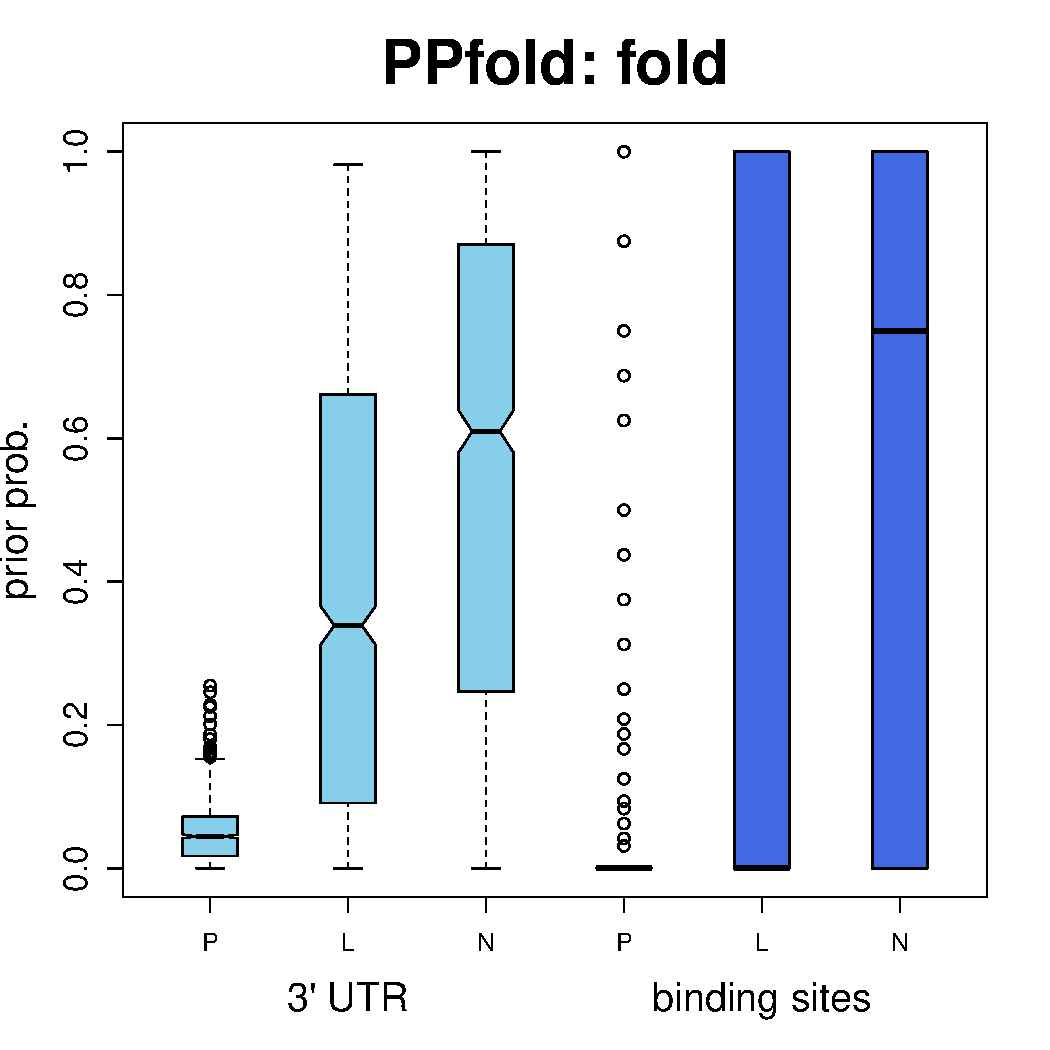
\includegraphics[width = 0.6\textwidth]{pfold_fd_npl_group}
    \caption[PPfold: Boxplot of structural annotation probabilities for protein binding sites and 3'UTR.]{\label{fig5} Boxplot of structural annotation probabilities for Pumilio binding sites positions and 3'UTR positions. The structural annotations are generated by PPfold for each alignment position. Next, for positions within binding sites region and those in background region (3'UTR) of a transcript, the frequencies for N,P,L categories are used as probabilities. For each transcript, the probabilities are then plotted for comparison.}
  \end{center}
\end{figure}

\begin{figure}[!hbp]
  \begin{center}
    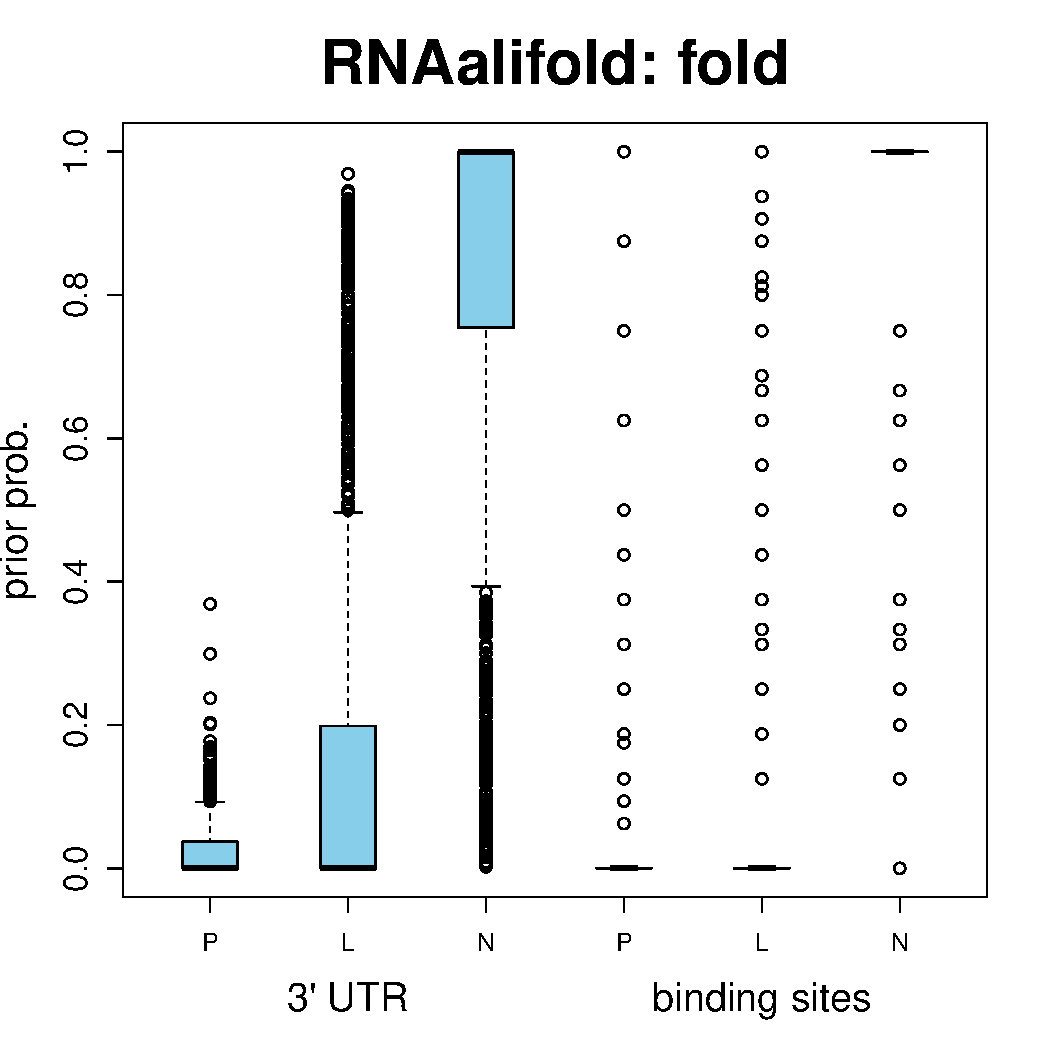
\includegraphics[width = 0.6\textwidth]{alifold_fd_npl_group}
    \caption[RNAalifold: Boxplot of structural annotation probabilities for protein binding sites and 3'UTR.]{\label{fig6} Boxplot of structural annotation probabilities for Pumilio binding sites positions and 3'UTR positions. The structural annotations are generated by RNAalifold for each alignment position. Next, for positions within binding sites region and those in background region (3'UTR) of a transcript, the frequencies for N,P,L categories are used as probabilities. For each transcript, the probabilities are then plotted for comparison.}
  \end{center}
\end{figure}

\FloatBarrier






\subsection{Motif-wise accessibility}
As described at the beginning of this chapter, for \textbf{motif-wise accessibility}, we look at each motif as a whole rather than consider single base. Similar to base-wise accessibility, we compare the motifs and background regions in "scan" and "fold" modes with N,P,L classification. Compared to base-wise accessibility, the motif-wise accessibility provides more detailed information of the pairing probability distribution on binding motif and background 3'UTRs, which is more important.

In the study of \cite{Li01062010}, the motif-wise accessibility is computed naturally by RNAplfold: consider the probability of the motif being single stranded in all Boltzmann distributed structures. As we would like to compare with RNAplfold using our comparative methods, we compute such motif-wise accessibility by taking average of the accessibilities of all single bases on a motif. We consider RBPs in all three species. Since there are too many of RBPs, only a subset of representative proteins in Yeast is shown below.



\subsubsection{"Scan" mode}
Similar to the definition in previous section, the "Scan" mode here is to assign a pairing probability to a sub-string that contains multiple consecutive bases. So $P(Pairing) = Prob_{avg}^b =$ (sum of pairing probabilities for all binding sites in a motif)/(number of the binding sites in that motif), and $Accessibility = 1 - P(Pairing)$.

First we look at the motif level accessibility on a simple case. As shown in Table~\ref{RBPs}, Msl5 motif does not occur very frequent in the Yeast UTR regions, so each of the transcript's UTR contains at most one hit of the motif Figure~\ref{decoderMsl5asAcc}.

\FloatBarrier
\begin{figure}[!hbp]
  \begin{center}
    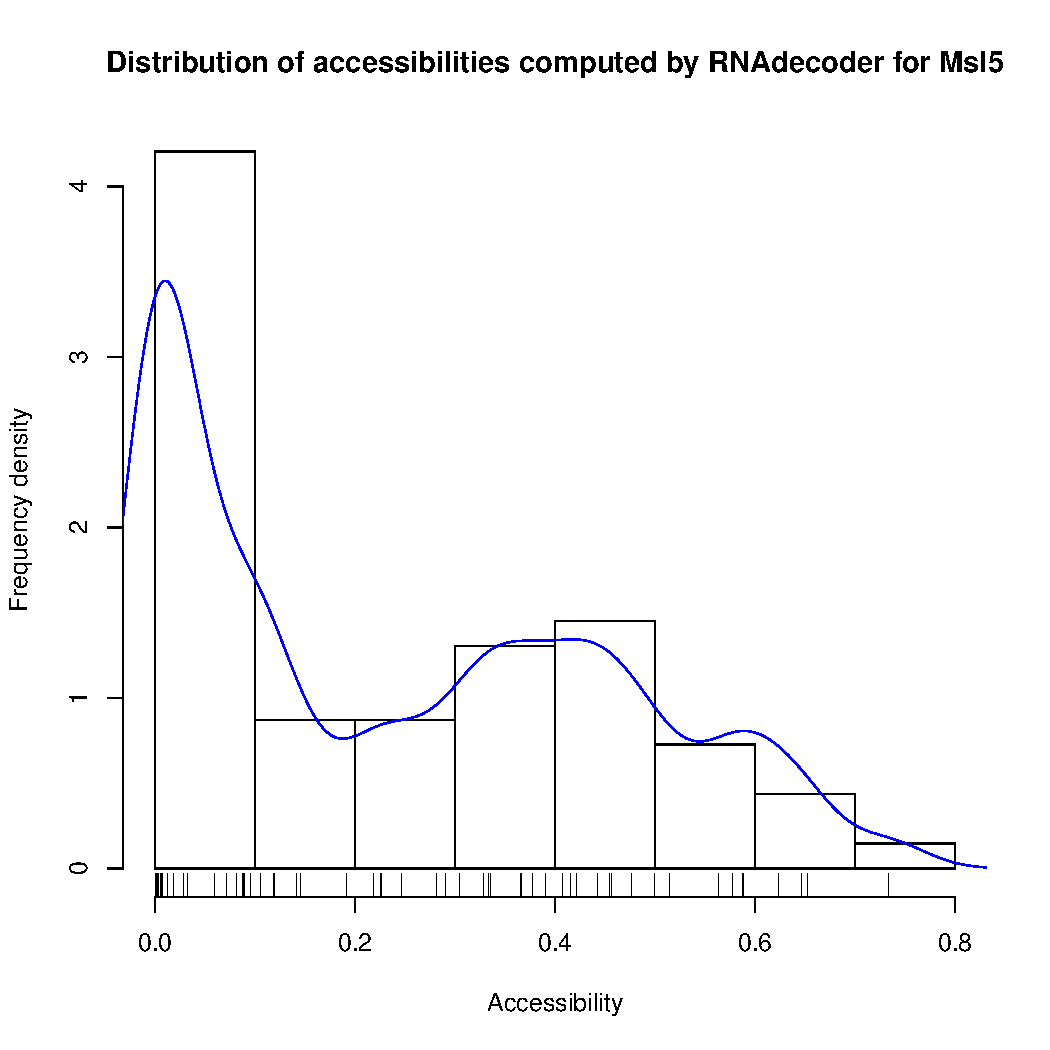
\includegraphics[width = 0.95\textwidth]{DistAccDecoderMsl5} %{Msl5-motifWiseAbsoluteScale_bp_acc}
    \caption[RNAdecoder scan mode: Msl5 protein on absolute scale accessibility]{\label{decoderMsl5asAcc} \textbf{Distribution of accessibilities computed by RNAdecoder for Msl5 protein.} Histogram plot of Msl5 motif-wise accessibility. $Accessibility = 1 - Pairing = 1 - Prob_{avg}^b$. The base pairing probabilities are generated by RNA-decoder for each alignment position.}
  \end{center}
\end{figure}
\FloatBarrier

Puf2 motif occurs more frequent than Msl5 in the Yeast UTR regions, so there are transcripts containing more than one motif. So we have two plots here: one for those UTRs with single motif Figure~\ref{decoderPuf2asSingle}, one for UTRs with multiple motifs Figure~\ref{decoderPuf2asMultiple}. In the second case, we further plot that: for any given such UTR, the accessibility value for the best/worst accessible binding motif.

As we can see, for those transcripts with single Puf2 motif in Figure~\ref{decoderPuf2asSingle}, the distribution is quite similar to Msl5 case in Figure~\ref{decoderMsl5asAcc}. And for those UTRs with multiple Puf2 binding motifs, the best accessible motifs are better than the worst motifs at a wide range, with a weak concentration at $worst = (0.25, 0.5)$ region as shown in Figure~\ref{decoderPuf2asMultiple}.

\FloatBarrier
\begin{figure}[!hbp]
  \begin{center}
    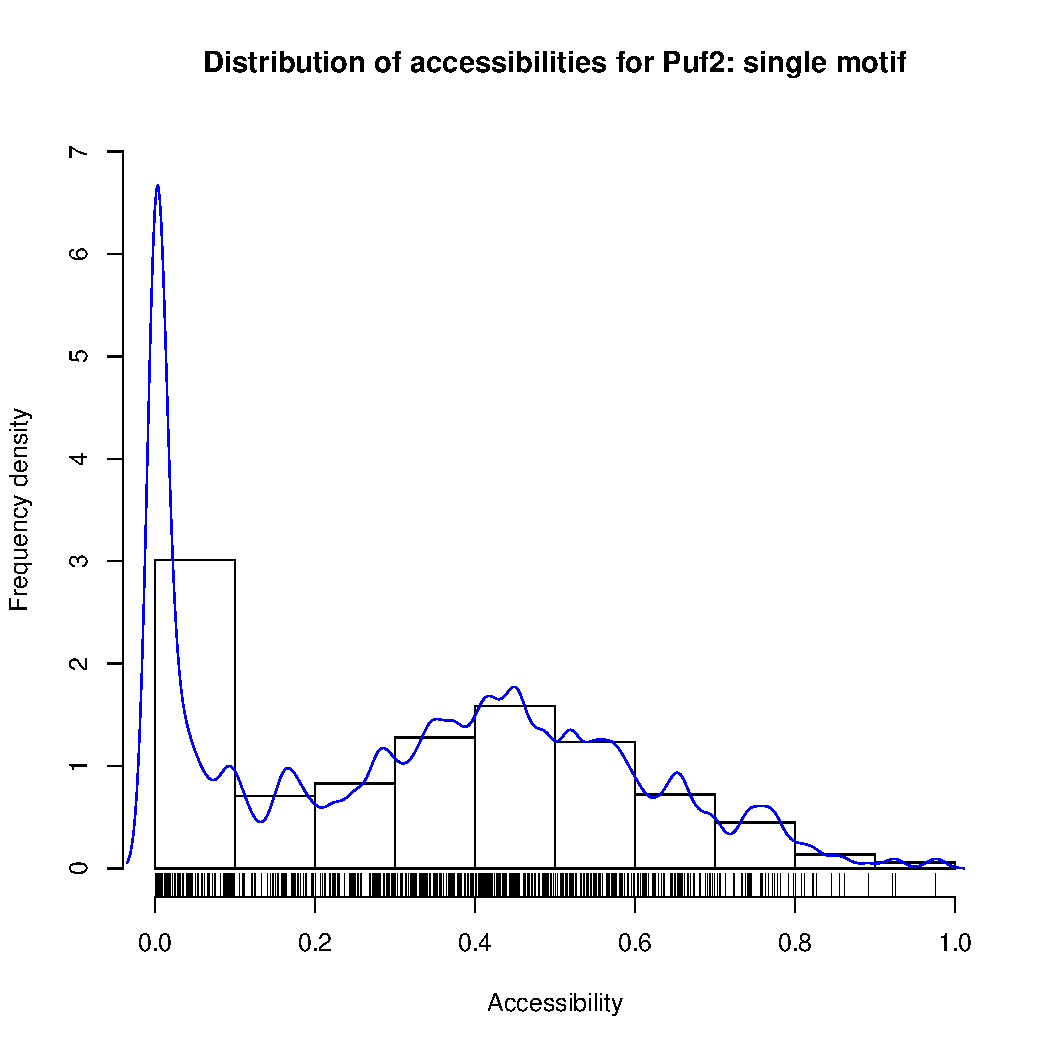
\includegraphics[width = 0.95\textwidth]{DistAccDecoderPuf2}
    \caption[RNAdecoder scan mode: Puf2 protein on absolute scale single motif]{\label{decoderPuf2asSingle} \textbf{RNAdecoder: Puf2 single motif accessibility distribution.} Histogram plot of Puf2 single motif accessibility. The figure is for those UTRs with single motif. $Accessibility = 1 - Pairing = 1 - Prob_{avg}^b$. The base pairing probabilities are generated by RNA-decoder for each alignment position.}
  \end{center}
\end{figure}

\begin{figure}[!hbp]
  \begin{center}
    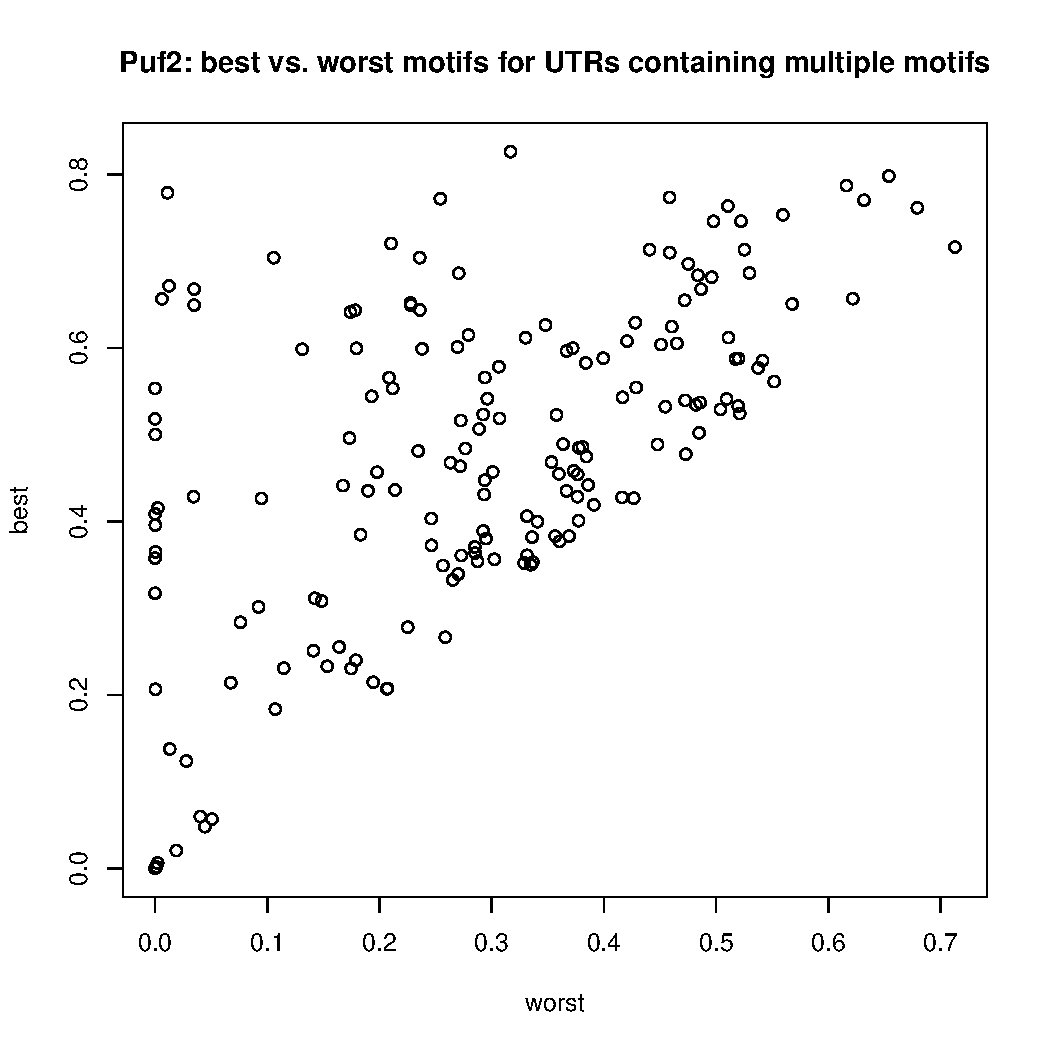
\includegraphics[width = 0.95\textwidth]{Puf2-motifWiseAbsoluteScale_bp_worstVSbest_plot}
    \caption[RNAdecoder fold mode: Puf2 protein on absolute scale multiple motifs]{\label{decoderPuf2asMultiple} \textbf{RNAdecoder: best vs. worst Puf2 motifs for UTRs containing multiple binding motifs.} Scatter plot of Puf2 multiple motifs accessibility. Each dot in the plot represents a UTR that contains multiple Puf2 binding motifs. The coordinates of any dot are $(worst, best)$, where $worst=Accessibility_{min}^b$, and similarly $best=Accessibility_{max}^b$. The structural annotations are generated by RNA-decoder for each alignment position.}
  \end{center}
\end{figure}
\FloatBarrier






\subsubsection{"Fold" mode}
As defined in previous section, the "Fold" mode is to assign a sequence of consensus label (one out of N,L,P) to a base. While here, we consider the N,L,P compositions in a binding motif. Also, we look at the differences between individual binding motif and its background UTR. Unlike in "Scan" mode, the detailed computation of the probabilities are different among the three programs. The below figures (Fig~\ref{fig24}, Fig~\ref{fig25} and Fig~\ref{fig26}) show such differences on an example protein Puf3-1. We could observe most of the dots are in quadrant 3 (bottom left) in PPfold and RNAalifold cases while for RNAdecoder the dots are more equally scattered. Still, this could be due to the fact that PPfold and RNAalifold tend to predict less structures (so less pairing and loop) than RNAdecoder.


\FloatBarrier

\begin{figure}[!hbp]
  \begin{center}
    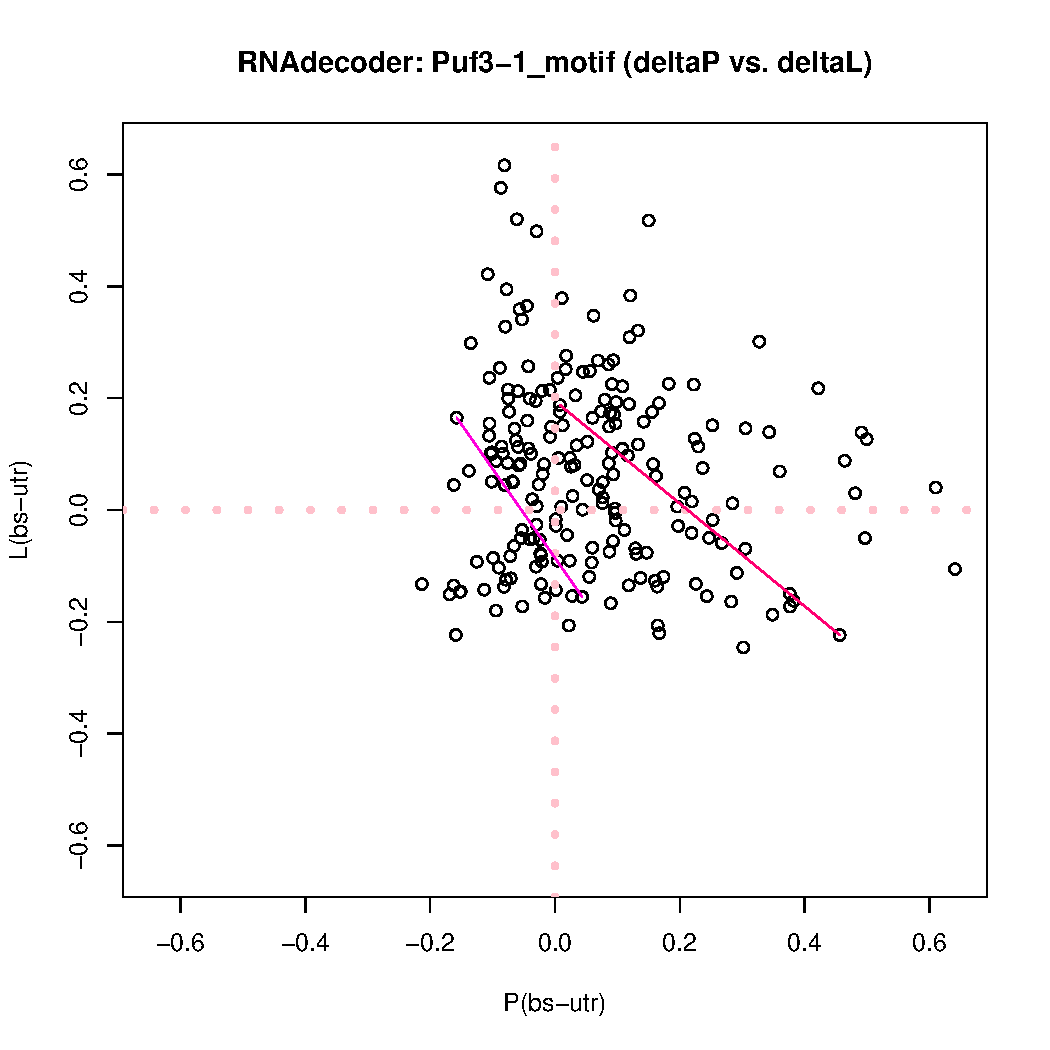
\includegraphics[width = 0.95\textwidth]{Puf3-1-motifWiseVSutrWise_fd_pVSl-decoder}
    \caption[RNAdecoder fold mode: Puf3-1 protein, motif VS UTR]{\label{fig24}  {Scatter plot of structural annotation probabilities for L vs P, in RNAdecoder case.} Each dot in the plot represents the difference between a Puf3-1 protein binding motif and its UTR. So the coordinates of any dot are $(\Delta P, \Delta L)$, where $\Delta P=P_{avg}^b - P_{avg}^U$ with $P_{avg}^b =$ (sum of likelihoods for binding sites labeled with P)/(length of the binding motif), and similarly $\Delta L=L_{avg}^b - L_{avg}^U$. The structural annotations are generated by RNA-decoder for each alignment position. Since one UTR may contain more than one binding motif, we use lines with the same colour to connect dots from the same UTR.}
  \end{center}
\end{figure}

\begin{figure}[!hbp]
  \begin{center}
    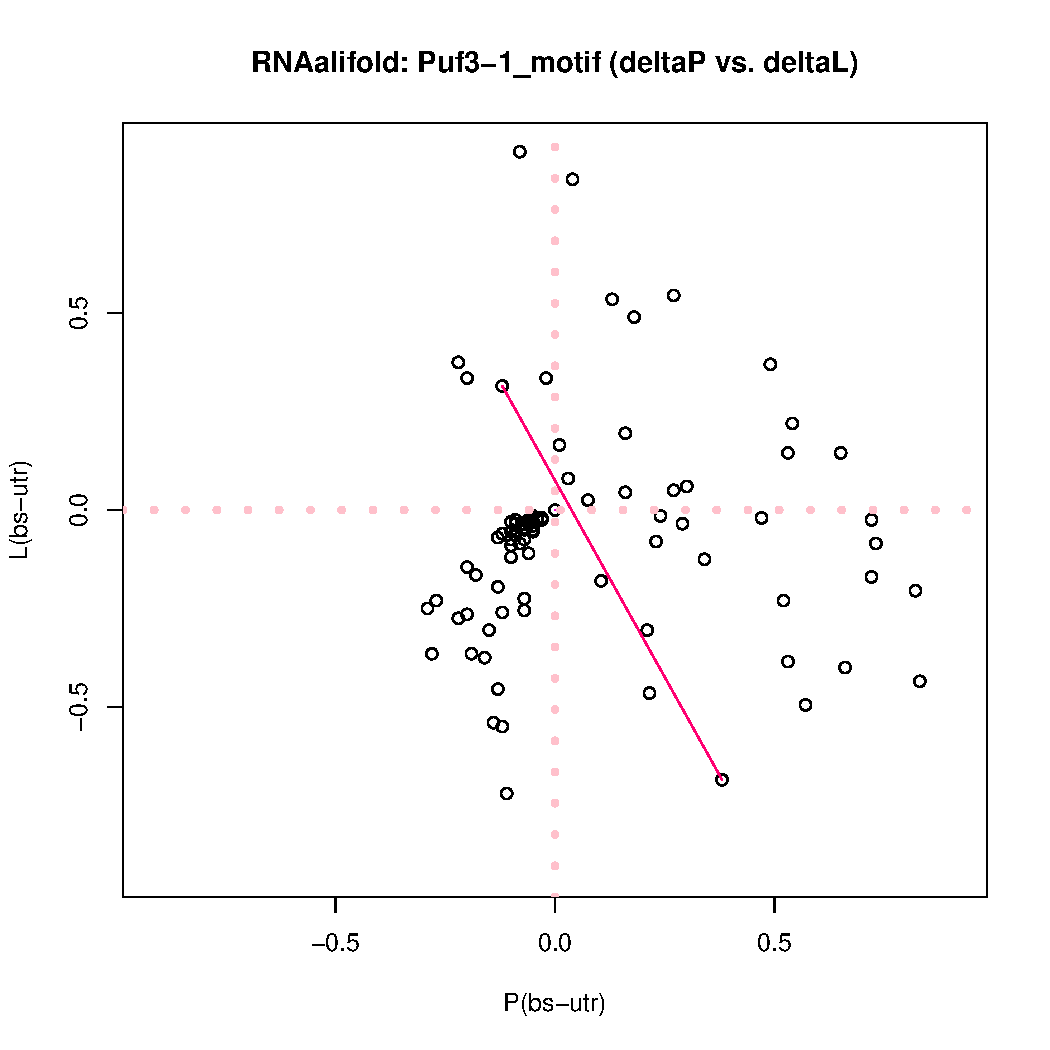
\includegraphics[width = 0.95\textwidth]{Puf3-1-motifWiseVSutrWise_fd_pVSl-alifold}
    \caption[RNAalifold fold mode: Puf3-1 protein, motif VS UTR]{\label{fig25} Scatter plot of structural annotation probabilities for L vs P. Each dot in the plot represents the difference between a Puf3-1 protein binding motif and its UTR. So the coordinates of any dot are $(\Delta P, \Delta L)$, where $\Delta P=P_{avg}^b - P_{avg}^U$ with $P_{avg}^b =$ (count of binding sites labeled with P)/(length of the binding motif), in RNAalifold case, and similarly $\Delta L=L_{avg}^b - L_{avg}^U$. The structural annotations are generated by RNAalifold for each alignment position. Since one UTR may contain more than one binding motif, we use lines with the same colour to connect dots from the same UTR. Note that the other line is not shown in this figure as that UTR is too long for RNAalifold to compute.}
  \end{center}
\end{figure}

\begin{figure}[!hbp]
  \begin{center}
    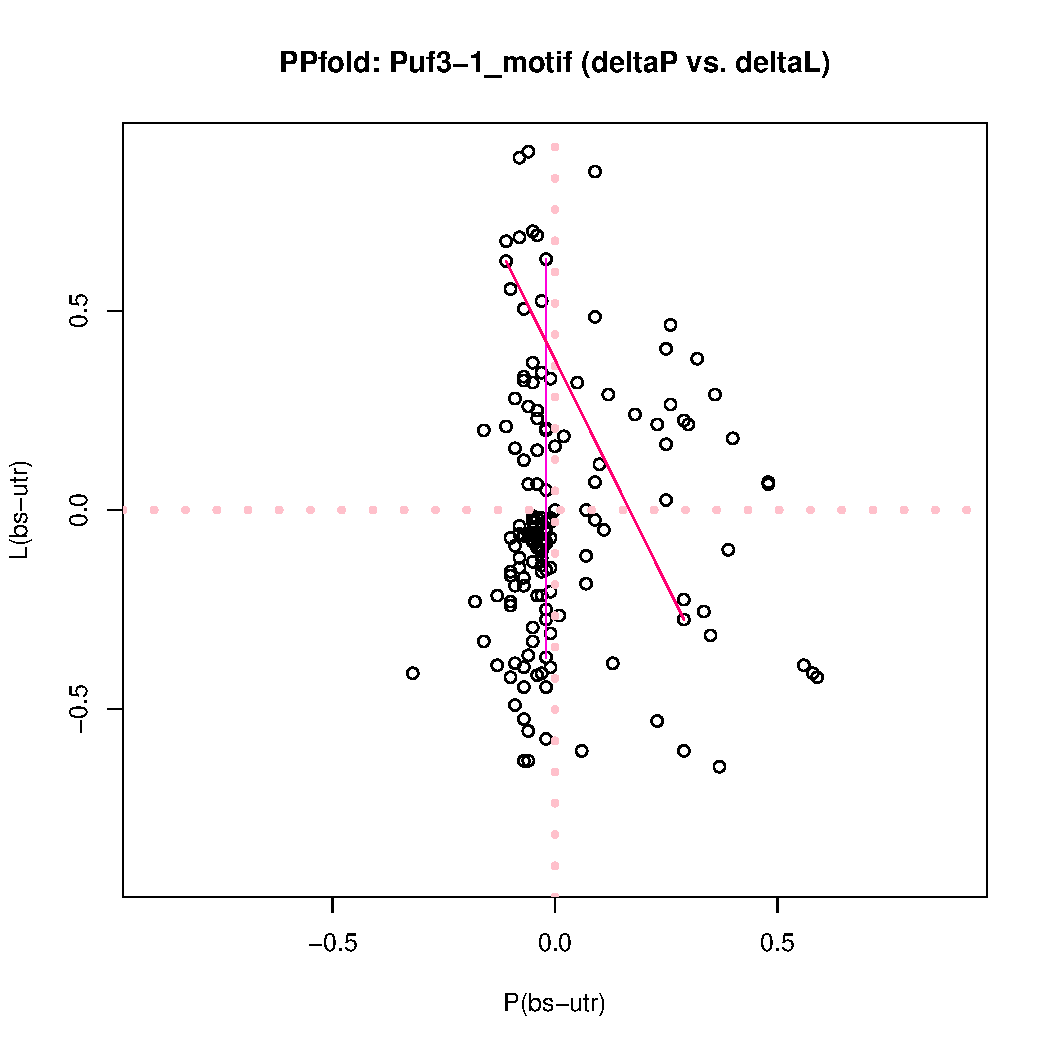
\includegraphics[width = 0.95\textwidth]{Puf3-1-motifWiseVSutrWise_fd_pVSl-ppfold}
    \caption[PPfold fold mode: Puf3-1 protein, motif VS UTR]{\label{fig26} Scatter plot of structural annotation probabilities for L vs P, in PPfold case. Each dot in the plot represents the difference between a Puf3-1 protein binding motif and its UTR. So the coordinates of any dot are $(\Delta P, \Delta L)$, where $\Delta P=P_{avg}^b - P_{avg}^U$ with $P_{avg}^b =$ (count of binding sites labeled with P)/(length of the binding motif), and similarly $\Delta L=L_{avg}^b - L_{avg}^U$. The structural annotations are generated by PPfold for each alignment position. Since one UTR may contain more than one binding motif, we use lines with the same colour to connect dots from the same UTR.}
  \end{center}
\end{figure}
\FloatBarrier


Besides, since RNAdecoder is the only one program among the three that can calculate the likelihood for each assigned structural label, we further look at the N,P,L distribution within binding motifs, as shown in figures Fig~\ref{decoderMsl5asLNvsP}, Fig~\ref{decoderMsl5asLvsP} and Fig~\ref{decoderMsl5asNvsP}. As we could see from Figure~\ref{decoderMsl5asLvsP} and Fig~\ref{decoderMsl5asNvsP}, the probability of either L or N alone is relatively lower than P. But when considering L$+$N, the probability is comparable to P as shown in Fig~\ref{decoderMsl5asLNvsP}.


\FloatBarrier

\begin{figure}[!hbp]
  \begin{center}
    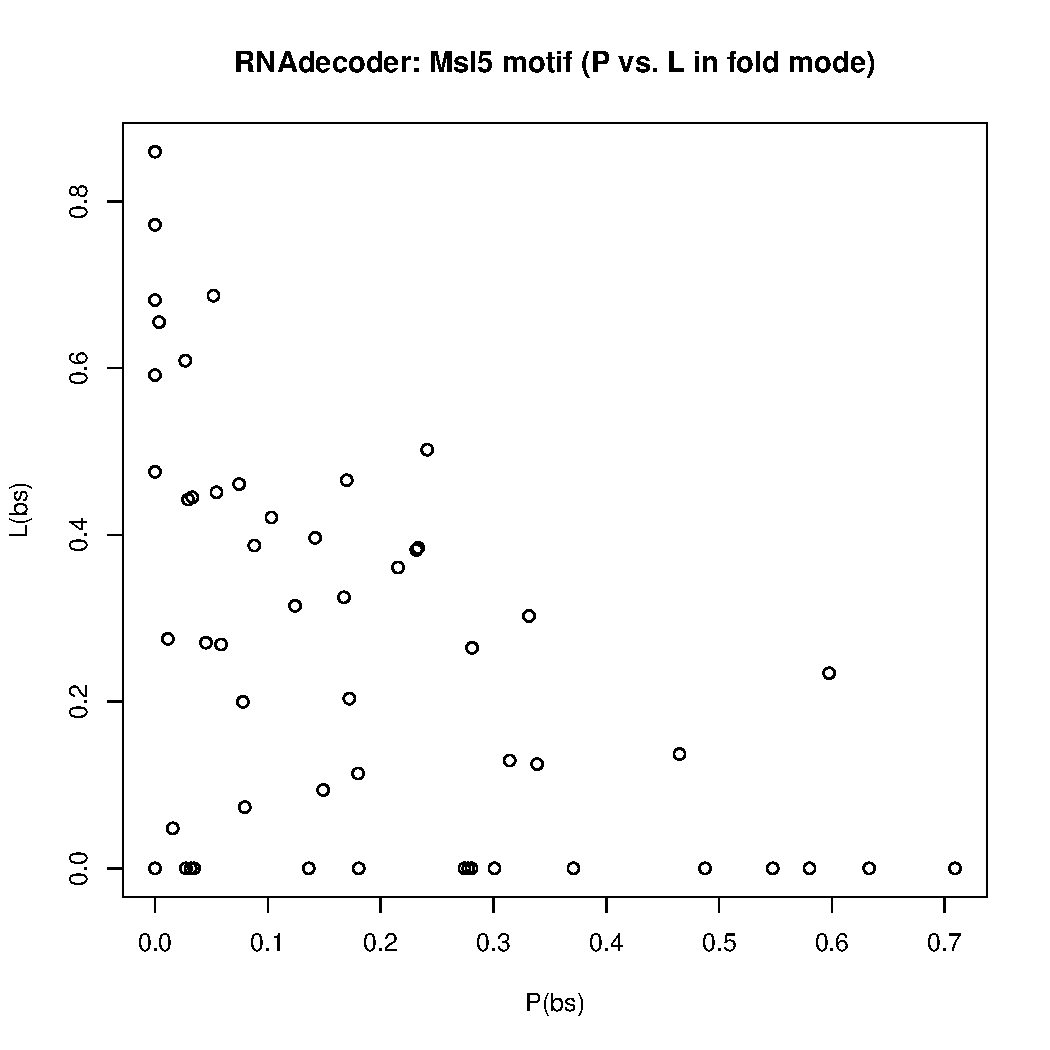
\includegraphics[width = 0.95\textwidth]{Msl5-motifWiseAbsoluteScale_fd_pVSl_plot}
    \caption[RNAdecoder fold mode: Msl5 protein P vs L]{\label{decoderMsl5asLvsP} \textbf{RNAdecoder: Msl5 motif (P vs. L) on absolute scale.} Scatter plot of structural annotation probabilities for L vs P, in RNAdecoder case. Each dot in the plot represents a Msl5 protein binding motif. So the coordinates of any dot are $(P, L)$, where $P=P_{avg}^b=$ (sum of likelihoods for binding sites labeled with P)/(length of the binding motif), and similarly $L=L_{avg}^b$. The structural annotations are generated by RNA-decoder for each alignment position.}
  \end{center}
\end{figure}

\begin{figure}[!hbp]
  \begin{center}
    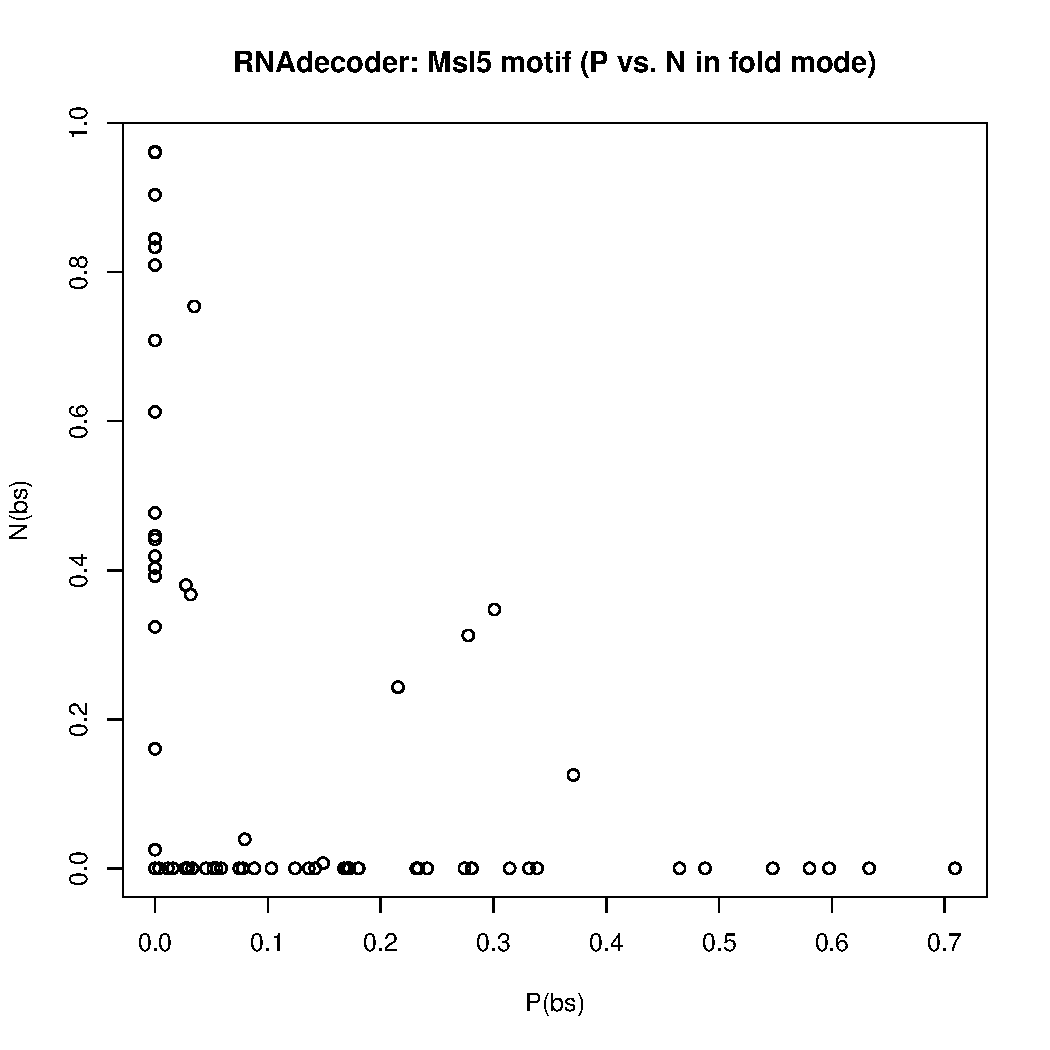
\includegraphics[width = 0.95\textwidth]{Msl5-motifWiseAbsoluteScale_fd_pVSn_plot}
    \caption[RNAdecoder fold mode: Msl5 protein on P vs N]{\label{decoderMsl5asNvsP} \textbf{RNAdecoder: Msl5 motif (P vs. N) on absolute scale.} Scatter plot of structural annotation probabilities for N vs P, in RNAdecoder case. Each dot in the plot represents a Msl5 protein binding motif. So the coordinates of any dot are $(P, N)$, where $P=P_{avg}^b=$ (sum of likelihoods for binding sites labeled with P)/(length of the binding motif), and similarly $N=N_{avg}^b$. The structural annotations are generated by RNA-decoder for each alignment position.}
  \end{center}
\end{figure}


\FloatBarrier
\begin{figure}[!hbp]
  \begin{center}
    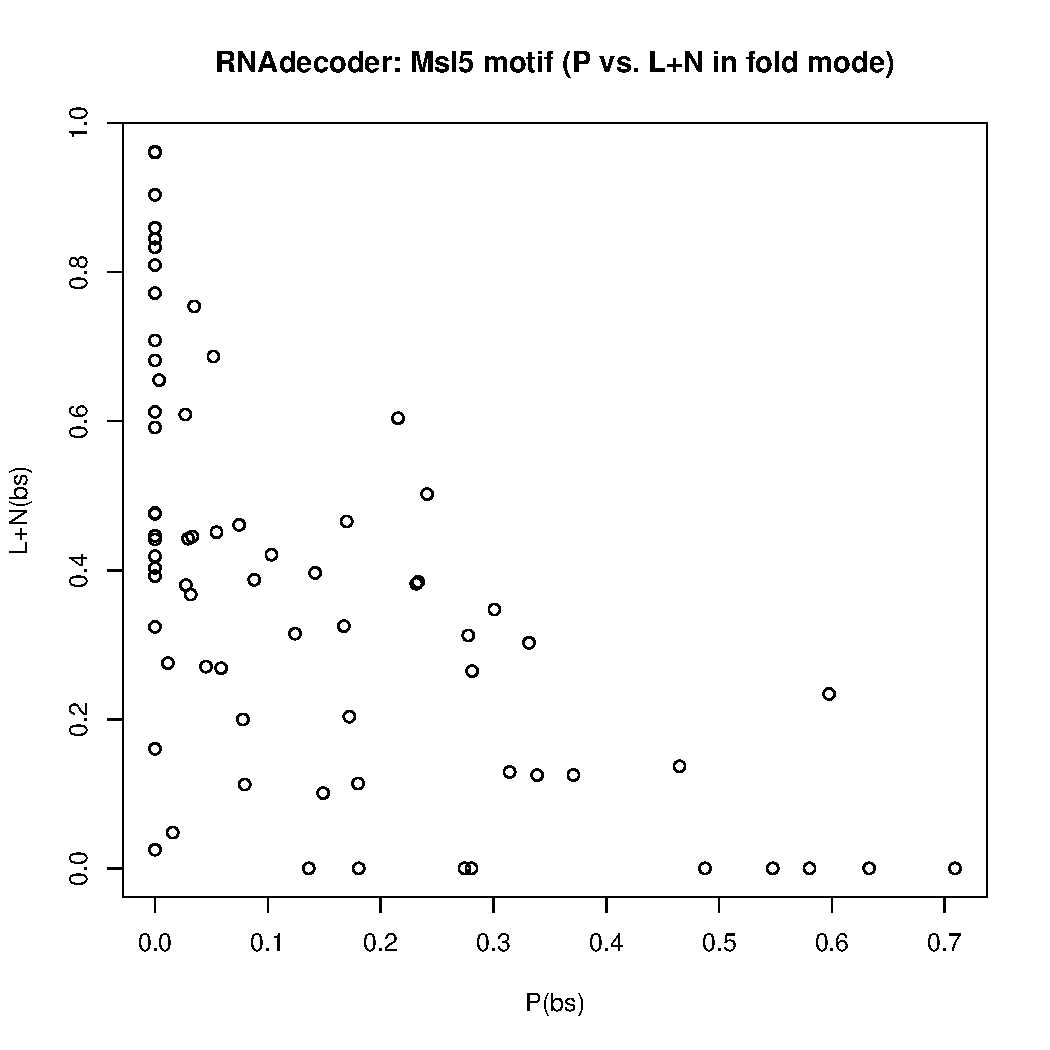
\includegraphics[width = 0.95\textwidth]{Msl5-motifWiseAbsoluteScale_fd_pVSln_plot}
    \caption[RNAdecoder fold mode: Msl5 protein P vs LN]{\label{decoderMsl5asLNvsP} \textbf{RNAdecoder: Msl5 motif (P vs. L+N) on absolute scale.} Scatter plot of structural annotation probabilities for L+N vs P, in RNAdecoder case. Each dot in the plot represents a Msl5 protein binding motif. So the coordinates of any dot are $(P, L+N)$, where $P=P_{avg}^b=$ (sum of likelihoods for binding sites labeled with P)/(length of the binding motif), and similarly $L+N=L_{avg}^b + N_{avg}^b$. The structural annotations are generated by RNA-decoder for each alignment position.}
  \end{center}
\end{figure}


\FloatBarrier






\subsection{Visualization of the alignment, structural annotation and accessibility}
By all means, it would be very useful if we could visualize the structural context around the binding motif on 3'UTR region. This section presents our progress on this task.

\subsubsection{Motif logo}
Motif-wise accessibility with regarding to NLP distribution could be shown independently as motif logo in Figure~\ref{fig17}. However, such figure does not give much useful information as "N" is the dominant case for every position. It would be better to put the binding sites motif back to the sequence context to get an idea of how different it is compared to other non-binding region.

\begin{figure}[!hbp]
  \begin{center}
    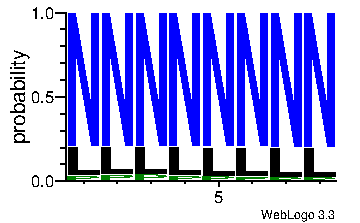
\includegraphics[width = 0.6\textwidth]{alifold_NPL_motifWise_fd}
    \caption[Motif logo for Pumilio by RNAalifold.]{\label{fig17} This is the motif logo for Pumilio (UGUAHAUA) protein of Fly, predicted by RNAalifold.}
  \end{center}
\end{figure}
\FloatBarrier



\subsubsection{More advanced visualization}
In order to visualize predictions from "fold" and "scan" modes for individual binding sites in individual UTRs, a combination of berrylogo \cite{berrylogo} and our lab's R4RNA package is built (a perl script called ccPBS.pl).

A berryLogo is a seqLogo alternative developed by Charles C. Berry for \cite{berrylogo}. Instead of "information content", the y-axis is the log relative frequency with respect to the background frequency, generated originally from the gc\_content parameter. Based on the original version I re-coded my version to visualize predictions from "fold". Currently I have not used the background frequency yet.

R4RNA is used to draw the pairing probability (1-accessibility) from "scan". For berrylogo.r, the script uses ggplot2 which is using lattice and based on 'grid' graphics subsystem, while the original R programs including R4RNA use 'base' graphics system. Noted that it is fairly difficult to combine figures from different systems.

Moreover, in order to connect the plots codes from R and computation codes from Perl more efficiently, a perl module Statistics::R is set up so that one can not only pass R commands as inline script in Perl but also directly pass and retrieve scalars or arrays variables between these two languages.

Given the transcripts ID, protein name and program name (like RNAdecoder), ccPBS.pl could generate a pdf with plot for "scan" on top and plot for "fold" at bottom. Two examples are shown below in Figure~\ref{fig18} and Figure~\ref{fig19}

\FloatBarrier
\begin{figure}[!hbp]
  \begin{center}
    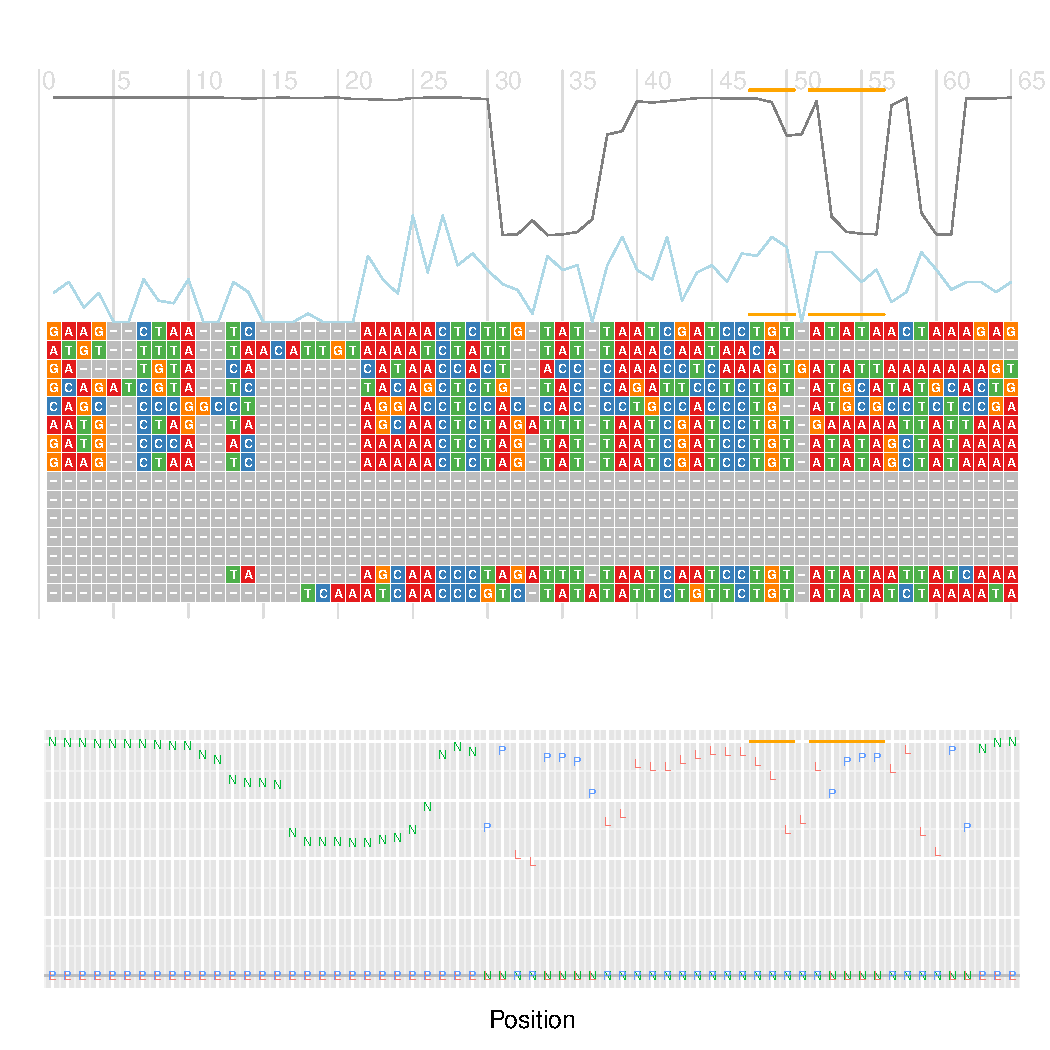
\includegraphics[width = \textwidth]{FBtr0078004_decoder_Pumilio_flyV2}
    \caption[Sequence wise visualization of FBtr0078004\_decoder\_Pumilio\_fly]{\label{fig18} This is a figure based on the prediction results from RNAdecoder. RNA: the 3'UTR of Fly FBtr0078004 transcript. Protein: Pumilio. 1). The plot on top is for "scan". Above the alignment, the grey line shows the pairing probability for each position. The binding sites regions are highlighted in yellow (on the grey line). The blue line shows the sequence conservation of the alignment. 2). The plot at bottom is for "fold". For each position, the N,L,P classifications are plotted according to their prior probabilities. Similarly, binding sites regions are highlighted as yellow fragments.}
  \end{center}
\end{figure}

\begin{figure}[!hbp]
  \begin{center}
    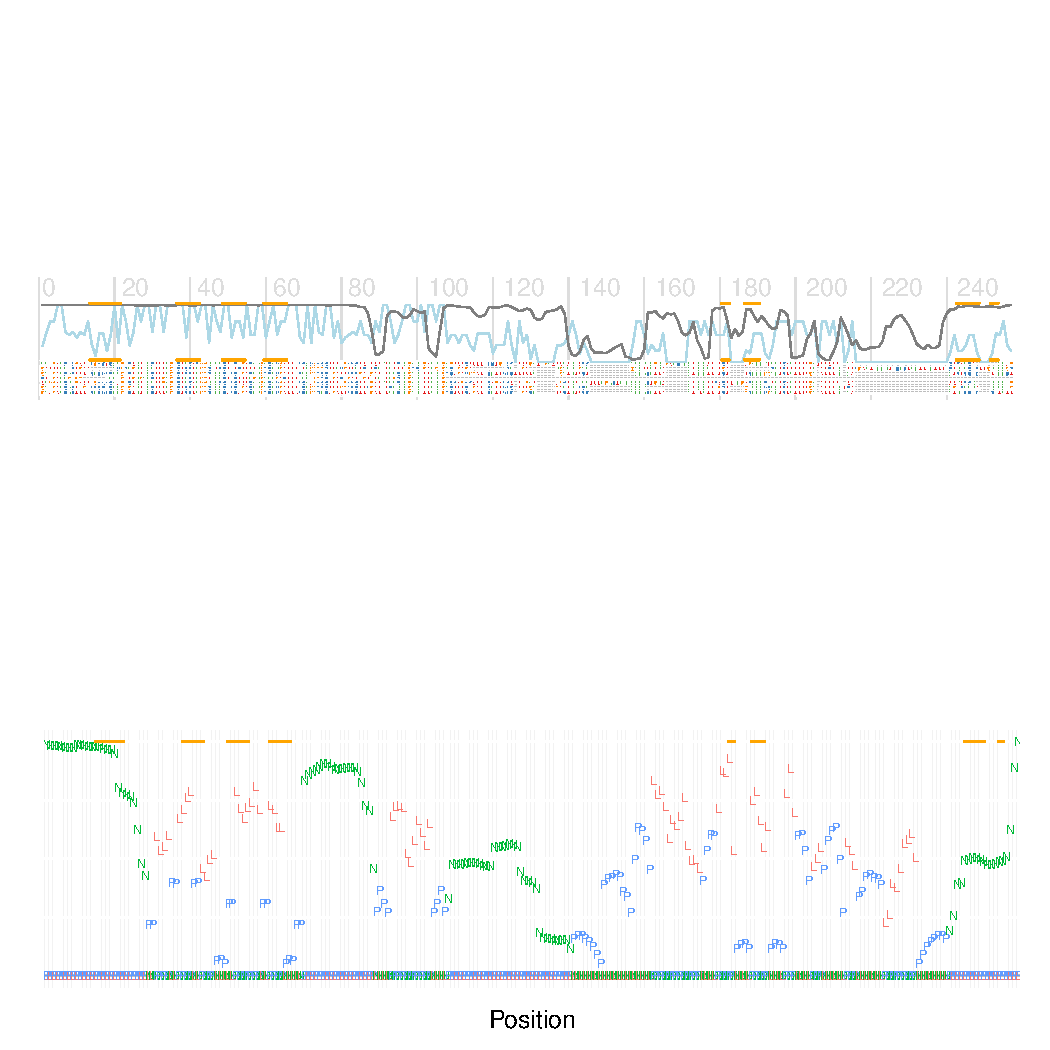
\includegraphics[width = \textwidth]{YAL001C_decoder_Khd1_yeastV2}
    \caption[Sequence wise visualization of YAL001C\_decoder\_Khd1\_yeast]{\label{fig19} This is another example based on the prediction results from RNAdecoder. RNA: the 3'UTR of Yeast YAL001C transcript. Protein: Khd1. It shows the case of a longer alignment with multiple binding motif hits.}
  \end{center}
\end{figure}
\FloatBarrier

Probably we could cluster the UTRs/binding sites according to their accessibility so that we may be able to visualize and see if there is any pattern for the binding sites.
For each potential binding motif (i.e. a sequence matching), we could get its pairing probability curve centered at the binding motif with flanking regions. And I found in several ENCODE papers, they have introduced how to cluster curves for features around TSS, like the paper \cite{Kundaje01092012}. Those features are mostly CHIP-seq signals or histone modification signals. In our case, we can easily change these to base pairing probabilities generated from those programs. And we could observe if there is any pattern surrounding binding motif by clustering these pairing signals.






\FloatBarrier
\section{Undergoing work}
\subsection{Realign the original alignment from UCSC}
\subsubsection{Structurally realign}
As shown in the previous section, the performances of the three programs we are using are highly depending on the quality of the input alignments. We propose to realign the raw 3'UTR alignments "cut" from UCSC whole genome alignments so that we would get more convincing results from those comparative methods. The original plan is to structurally realign them then compute the new accessibility.

There are programs like mlocarna and simulfold which can do realign and fold simultaneously. According to my labmate, Alborz's unpublished results, both programs are very slow, especially when the sequence length$>$1000; mlocarna is a bit faster in general. So I used mlocarna to realign Fly alignments at first place.

However, when I tested on a small set of alignments of Fly 3'UTRs, the program took hours to get the results. The main reason might be that the core part is a program called locarna which is used for pair-wise alignment, and mlocarna is a large perl script calls locarna for progressive alignment. Besides, the original authors of mlocarna suggests to use sequence-based realignment in their paper \cite{Andreas2012}. In that paper, they use mlocarna for sRNA realign and MAFFT for mRNA realign. So I take their suggestions here in my project.



\subsubsection{Sequence-based realign}
For sequence-based realignment, since Human species has the longest 3'UTR sequences and the largest alignment (44way) among all three species, I start from Human to build the computational pipeline.


\iffalse
\begin{longtable}{*{1}{p{35pt}}|*{1}{p{85pt}}|*{1}{p{40pt}}|*{1}{p{65pt}}|*{1}{p{120pt}}}%{lllll} %{{}{}{}{}{p{48pt}}}
\caption{\label{RBPs_human} Overview of Human RBPs in Li2010 paper.}

    \\
    \hline%\toprule
    \hline
    \textbf{RBPs}&\textbf{Motif}&\textbf{Binding type}&\textbf{Database ID}&\textbf{Database Info}\\
    \hline\hline%\midrule
    PTB & UCUUC, UCUU, YCU & & AAC99798 (NCBI) & polypyrimidine tract binding \\\hline
    HuR & NNUUNNUUU & & AAB41913 & Elav-like family; binds specifically to AU rich elements (AREs) in 3'UTRs \\\hline
    Pum1 & UGUAHAUA & & NP\_001018494 & Puf family \\   \hline\hline%\bottomrule
\end{longtable}
\fi


\paragraph{Pick the best set of species from UCSC MSAs}
\subparagraph{Binding proteins' homologs}
In order to control the quality of the MSA, the first thing is to make sure there are corresponding RBPs exist in all the species of the MSA as shown in Figure~\ref{tree44way}. So for each of those human RBPs listed in Table~\ref{RBPs_human}, we have searched for the homologs of its gene in NCBI.


\FloatBarrier
\begin{longtable}{*{1}{p{35pt}}|*{1}{p{85pt}}|*{1}{p{120pt}}}%{lllll} %{{}{}{}{}{p{48pt}}}
\caption{\label{RBPs_human} Human RBPs in our dataset.}

    \\
    \hline%\toprule
    \hline
    \textbf{RBPs}&\textbf{Database ID}&\textbf{Database Info}\\
    \hline\hline%\midrule
    PTB & AAC99798 (NCBI) & polypyrimidine tract binding \\\hline
    HuR & AAB41913 & Elav-like family; binds specifically to AU rich elements (AREs) in 3'UTRs \\\hline
    Pum1 & NP\_001018494 & Puf family \\   \hline\hline%\bottomrule
\end{longtable}

\FloatBarrier

For PTB, the human PTBP1 gene is conserved in chimpanzee, Rhesus monkey, dog, cow, mouse, rat, chicken, zebrafish, fruit fly, mosquito, C.elegans, A.thaliana, and rice.

For HuR, since it is a member of Elav-like family, the human ELAVL1 gene is conserved in chimpanzee, Rhesus monkey, dog, cow, mouse, rat, chicken, zebrafish, and C.elegans.

For Pum1, its human gene is conserved in chimpanzee, Rhesus monkey, dog, cow, mouse, rat, chicken, and zebrafish. Moreover, this gene encodes a member of the PUF family, evolutionarily conserved RNA-binding proteins related to the Pumilio proteins of Drosophila and the fem-3 mRNA binding factor proteins of C. elegans.

For all the species in the human 44way MSA, the most distant one (outgroup) from human is Petromyzon marinus. So we can conclude that it is safe to include all the 44 species in the MSA, from proteins' point of view.

We have also searched the three proteins in Treefam (using their NCBI ID to search against the DB). The results are basically the same. Besides, Treefam provides the orthologs family trees for each of the protein gene (not found it very useful since the species coverage is small), which are also consistent.

\subparagraph{Sequence similarity}
The phylogenetics tree for hg18 44way vertebrate MSA is downloaded from \href{ftp://hgdownload.cse.ucsc.edu/goldenPath/hg18/phastCons44way}{UCSC}. This tree as shown in Figure~\ref{tree44way} is used as the starting point. And the total tree length is: 12.117.

\FloatBarrier
\begin{figure}[!hbp]
  \begin{center}
    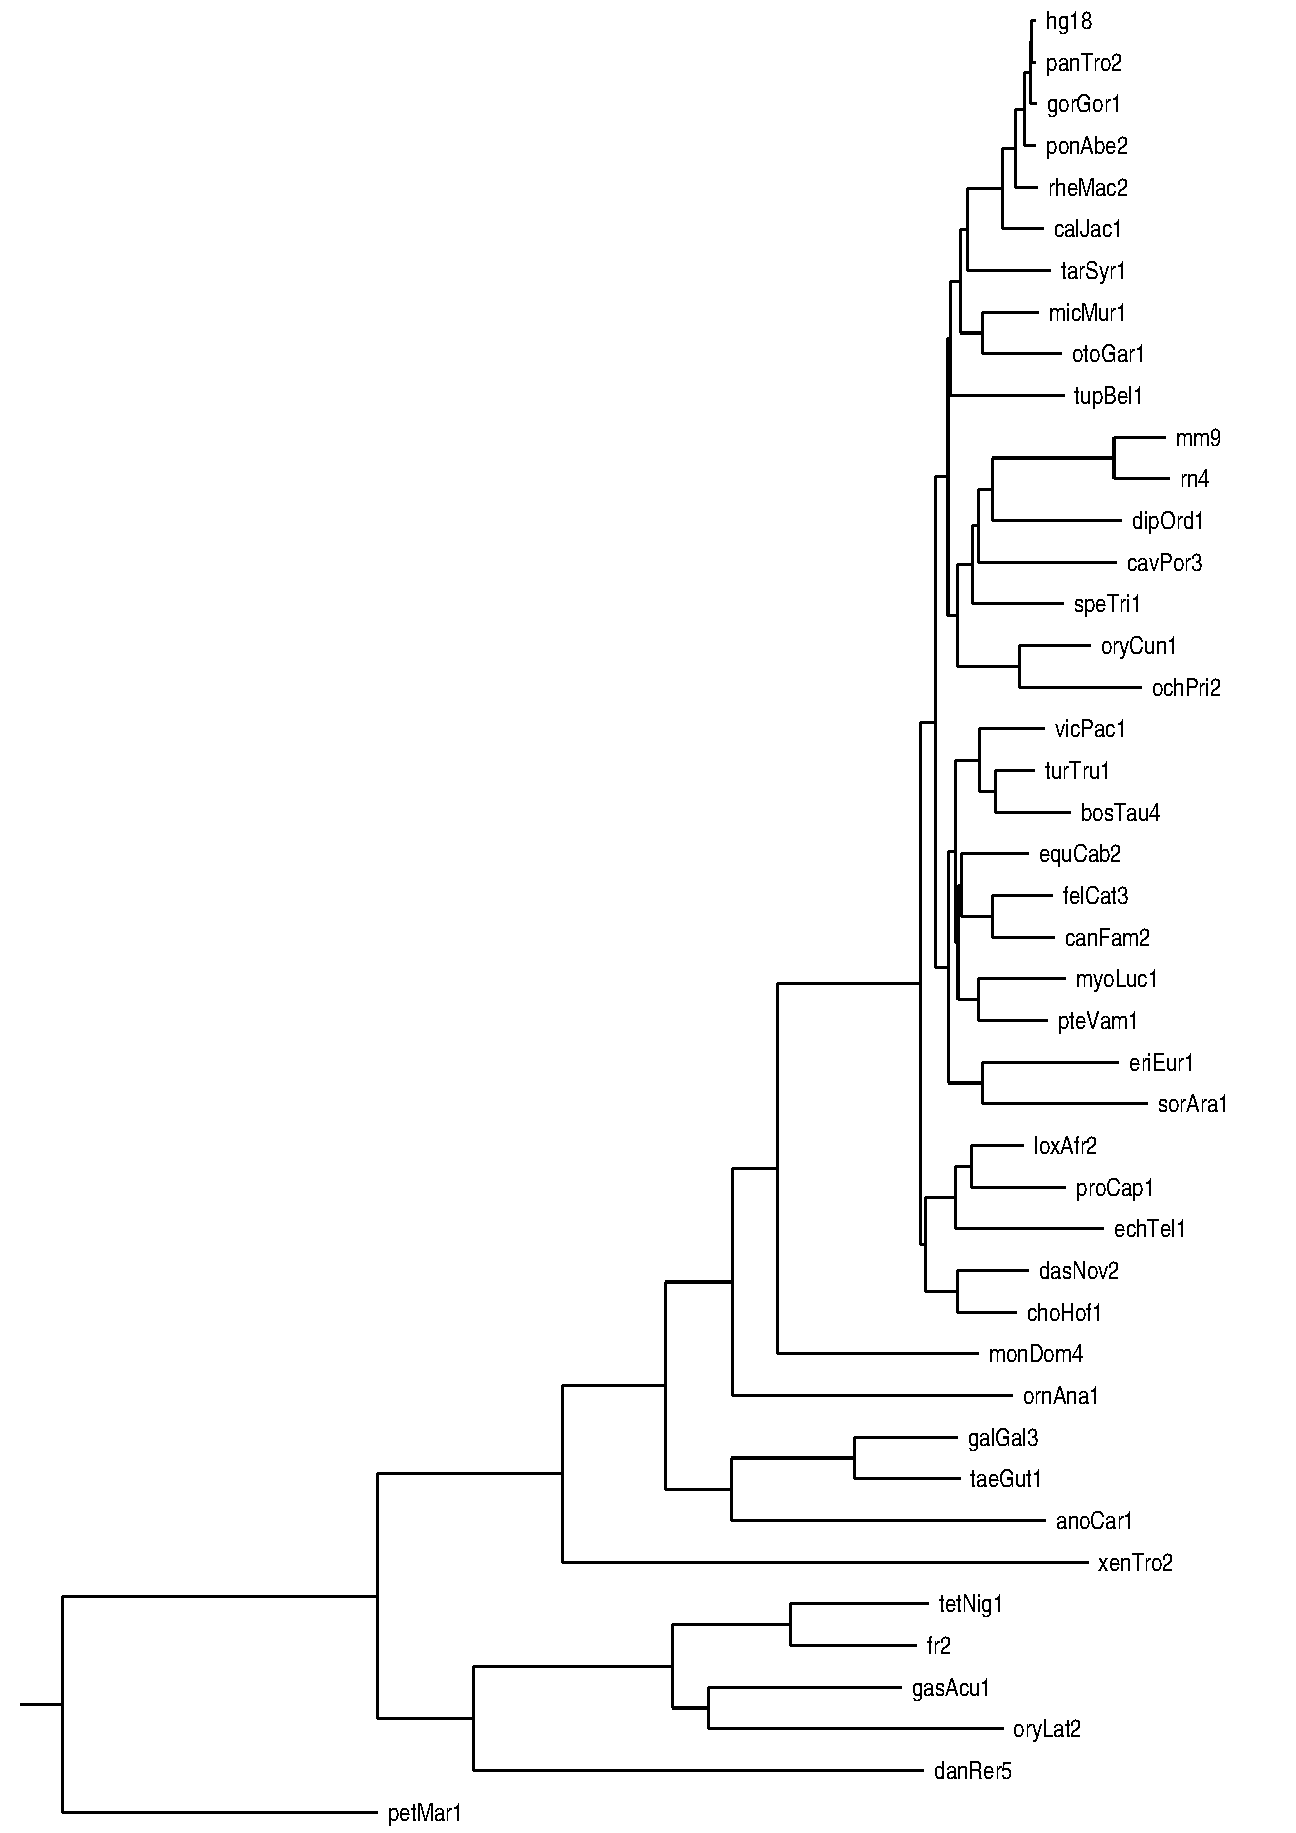
\includegraphics[height = 0.95\textheight]{vertebrate-eps-converted-to}
    \caption[Hg18 44way alignment: total tree]{\label{tree44way} Hg18 44way alignment: total tree. This figure is made based on \href{ftp://hgdownload.cse.ucsc.edu/goldenPath/hg18/phastCons44way}{UCSC} whole genome MSAs.}
  \end{center}
\end{figure}
\FloatBarrier

Next, we would like to get an idea of the distribution of tree length for human 3'UTR MSAs from UCSC. For any given MSA, we pick the overlapped species between it and the 44way tree. Then based on the 44way tree, the missing species are trimmed. Figure~\ref{ENST00000334314} shows an example of the 3'UTR MSAs for transcript ENST00000334314. Its total tree length is: 4.847.

\FloatBarrier
\begin{figure}[!hbp]
  \begin{center}
    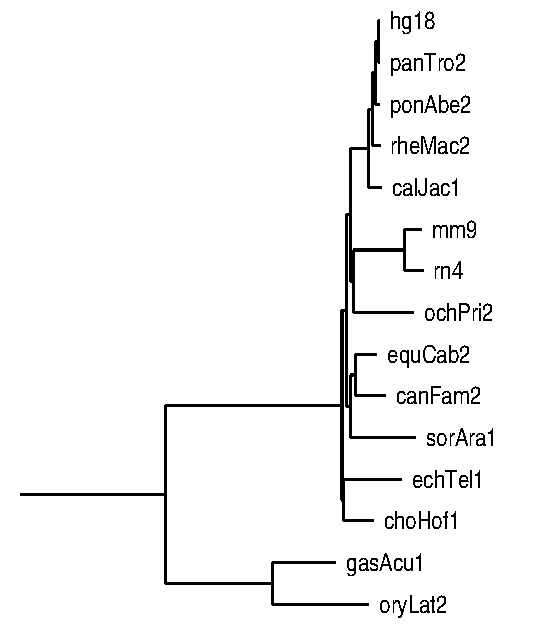
\includegraphics[height = 0.6\textheight]{ENST00000334314-eps-converted-to}
    \caption[ENST00000334314 alignment: 15way tree]{\label{ENST00000334314} ENST00000334314 alignment: 15way tree. This tree is pruned based on the 44way tree. Since for ENST00000334314 MSA, only 15 species out of 44 appear, the rest part of the 44way tree is pruned.}
  \end{center}
\end{figure}
\FloatBarrier

A randomly sampled subset (100 samples per chromosome) of all human 3'UTR MSAs is used to estimate the total tree length distribution of human 3'UTR alignments from UCSC. The results are shown as Figure~\ref{human3UTRtreeLenDist}. In summary, the mean length is 7.864 and median is 8.235.

\FloatBarrier
\begin{figure}[!hbp]
  \begin{center}
    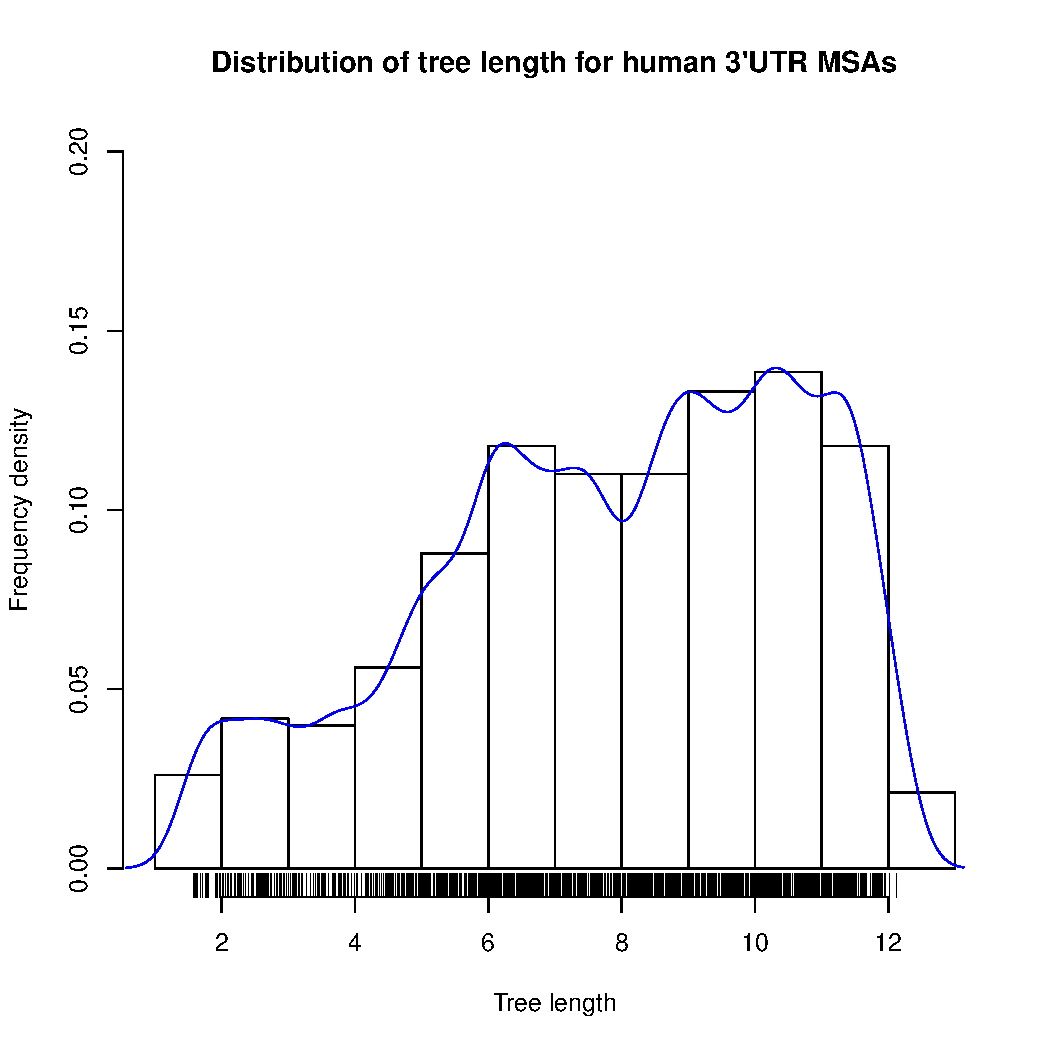
\includegraphics[width = \textwidth]{DistTreeLen}
    \caption[Distribution of total tree length for human 3'UTR MSAs]{\label{human3UTRtreeLenDist}Distribution of total tree length for human 3'UTR MSAs. The normalized frequency densities (y-xais) of different total tree lengths (x-xais) are shown. The bars at the bottom indicate the actual tree lengths.}
  \end{center}
\end{figure}
\FloatBarrier

Thus we would aim for a total tree length between 4 and 10 to get an appropriate MSA with regarding to evolutionary distance (sequence similarity).


Actually, the information of hg18 44way alignment is also listed as table at \href{http://genomewiki.ucsc.edu/index.php/Hg18_44way_alignment}{1} and \href{http://genomewiki.ucsc.edu/index.php/Genome_size_statistics}{2} . From the "\% of hg18 matched" column, we could see the matched percentage (i.e. alignment coverage) between human genome and each of the other 43 species. The rows have been sorted according to the percentage, as shown in Figure~\ref{Hg18Simi44way}.

\FloatBarrier
\begin{figure}[!hbp]
  \begin{center}
    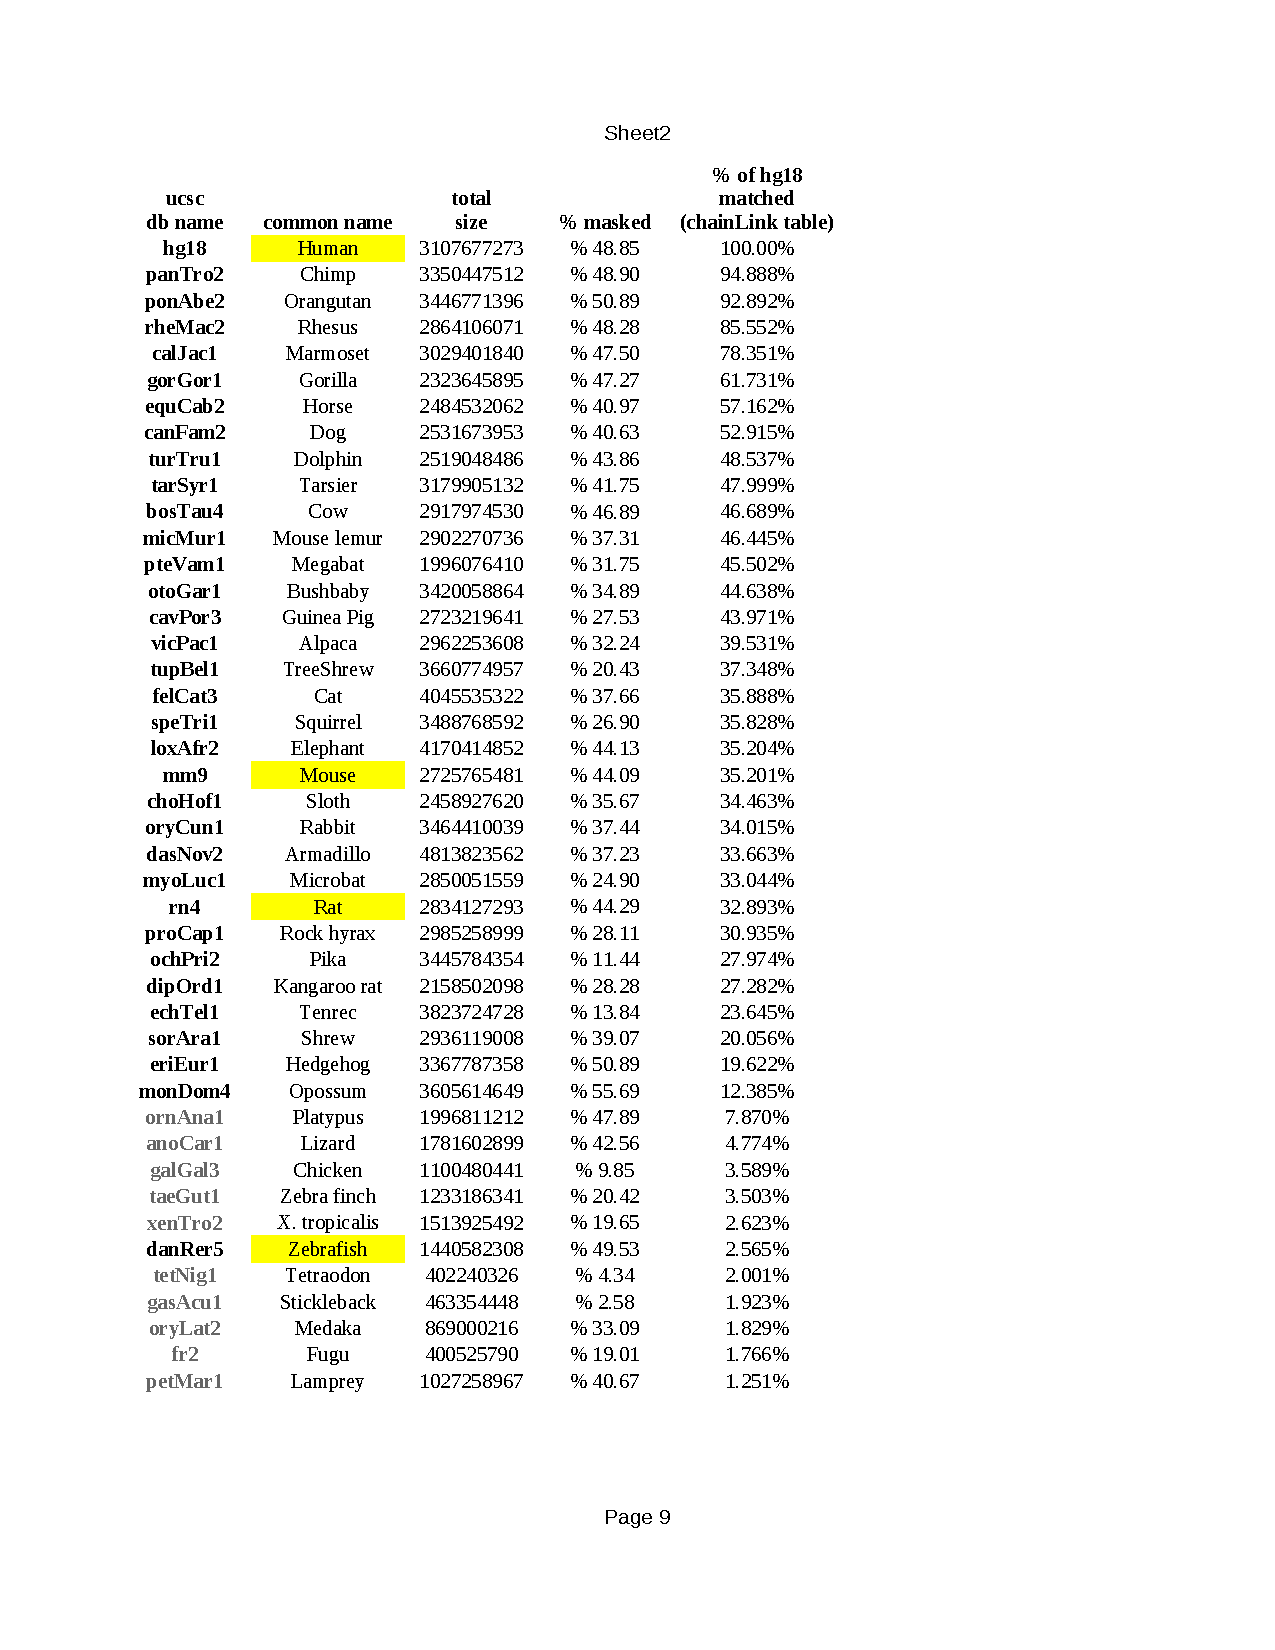
\includegraphics[height = 0.95\textheight]{Hg18Simi44way}
    \caption[Hg18 44way alignment: matched percentage]{\label{Hg18Simi44way}Hg18 44way alignment: matched percentage. This table is built based on the information from \href{http://genomewiki.ucsc.edu/index.php/Hg18_44way_alignment}{1} and \href{http://genomewiki.ucsc.edu/index.php/Genome_size_statistics}{2}. Note for the last column, the percentage is the alignment coverage rather than the evolutionary distance. Four widely studied model organisms (Human, mouse, rat, zebrafish) are highlighted.}
  \end{center}
\end{figure}
\FloatBarrier

So we can see that the rows below Opossum are all species with less than 10\% coverage to human. They are basically species which are the most distant from human. If we remove these species, the total tree length reduces to: 6.463. Even with the model organism zebrafish added, we have the tree length: 7.349.

However, as described above, for all the sampled human 3'UTRs the median tree length is 8.235. This means that the majority of the 3'UTRs have a relatively large coverage of the 44 species, including distant ones. So removing all of these distant species seems not to be a good idea.

Another way is to use K-means cluster algorithm to get the "rational" k representative species out of Figure~\ref{Hg18Simi44way}. A program has been implemented to parse table data using Algorithm::KMeans module. But still, the percentage values here could only be used to measure the distance to human. Even when two species have very close percentages to human, like elephant and mouse, it does not mean they should be clustered together.

Thus, the best way to control the quality for each 3'UTR MSA is really to do cluster on aligned sequences themselves, based on sequence similarity. A program called \textit{usearch} which is developed by the same author of MUSCLE is exactly for this job. That's what I plan to do in the next step.

But here, in order to get a general trimmed tree from the 44way whole genome tree, direct tree manipulating is needed. As described above, for all the three RBPs, all the 44 species are supposed to have homologs. So it is safe to select any one of the 44 species. Besides, there are some obvious clusters from  Figure~\ref{tree44way}. We could sample from each of the clusters according to the distances of its members. And this sampling may generate different trees (but their distance should be similar). At the moment, this process is done in a heuristic way: first generate the pair-wise distance matrix (attached), then fix hg18 and select tupBel1 which is the most distant one in that cluster, use the distance (D) between hg18 and tupBel1 as a criteria to select the following ones. It means the third one to join \{hg18, tupBel1\} is the one which is the most close to hg18 and tupBel1 among those nodes having distances to both hg18 and tupBel1 greater than D. And so is the fourth one.. In practice, this can be done using monophyly test which is implemented in Bio::Tree::Tree: given a set of nodes and a outgroup node, use is\_monophyletic() to test whether the common ancestor for the members of the internal\_nodes group is more recent than the common ancestor that any of them share with the outgroup node. So for each candidate node, the script loops over each of the rest nodes (excluding the candidate and those already selected) as the outgroup node. Based on this procedure, we could get the trimmed tree as Figure~\ref{tree23way}. And the total tree length is: 9.475. Note that setting the heuristic distance differently at the beginning would generate very different trees. Here, we basically reduce the number of nodes by half and keep almost the same diversity. So we would expect a less conserved alignment generated based on the trimmed tree.

\FloatBarrier
\begin{figure}[!hbp]
  \begin{center}
    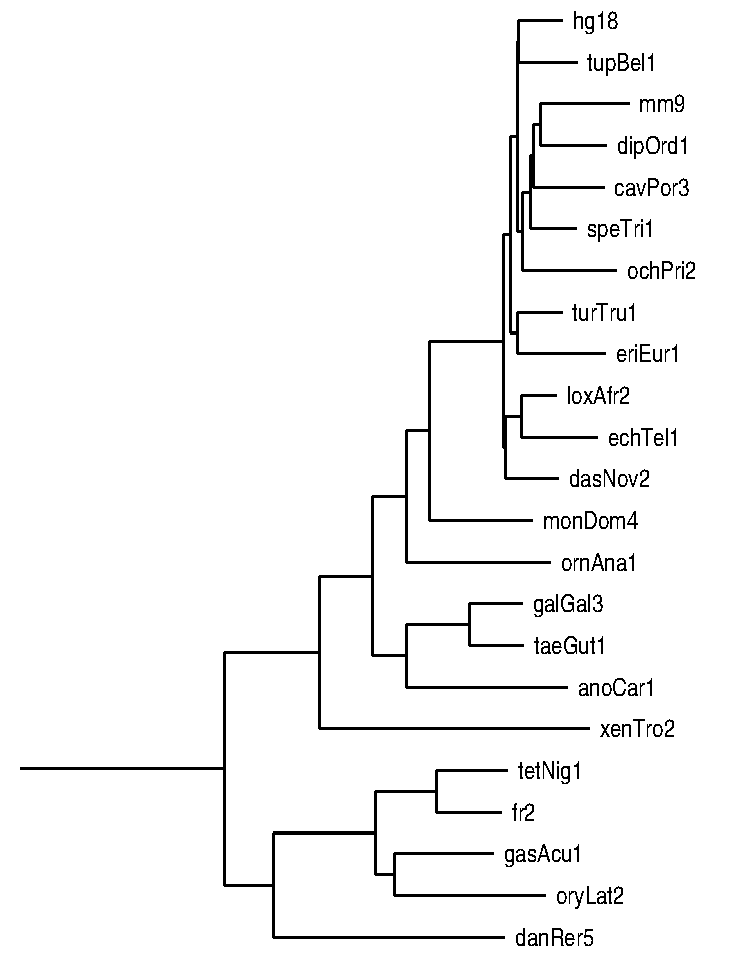
\includegraphics[height = \textheight]{23way-eps-converted-to}
    \caption[Hg18 23way alignment: trimmed tree]{\label{tree23way} Hg18 23way alignment: trimmed tree. This tree is built from the 44way tree from UCSC with quality control.}
  \end{center}
\end{figure}
\FloatBarrier

Actually if we could have more RBPs with diverse homologs ranges in the future, the best way might be to make a set of RBP-specific pruned trees. 


\paragraph{Realign MSAs for human 3' UTRs}
After getting the new tree, we would trim the MSA based on the tree. Given an MSA of some 3'UTR, a pipeline is built to get its overlapped entities with a designated tree, output the overlapped MSA and overlapped entities' tree (length, newick file, eps figure). As a result, any trimmed MSA with total tree length smaller than 4 or greater than 10 is removed.

As suggested in \cite{Andreas2012}, MAFFT is chosen to do the realignment based on sequence conservation. More specifically, as suggested by other labmates, MAFFT-einsi which is one of the three options in MAFFT (the other two are ginsi (for global aln) and linsi (for local aln). einsi is like the compromise between local and global) is used here.

The table below Table~\ref{realign_trimmed} shows the comparison between trimmed MSAs and raw UCSC MSAs re-alignments. The value in each cell is the average value across all 3'UTRs. It seems the trimmed 23way MSAs have worse conservation and more gaps. However, it highly depends on how to select the trimmed tree nodes. According to the method described above, the tree selected is more diverse compared to the raw one rather than conserve. We could see from the Figure~\ref{human3UTRtrimtreeLenDist}. The distribution of trimmed tree length is more concentrated in the 4 to 10 region. But the total tree length is still as high as 7.077 (Median, compared to 8.235 for the original), which indicates the variation is increasing.

\FloatBarrier


\begin{table}[ht]
  \begin{center}
    \begin{tabular}{|l||l|l||l|l|}
      \hline
      &\multicolumn{2}{l|}{Conservation}&\multicolumn{2}{l|}{Gappiness}\\
      \cline{2-5}
       &UCSC&\textbf{Realigned}&UCSC&\textbf{Realigned}\\
      \hline\hline
      23way& 0.397 &\textbf{0.411}& 0.521 &\textbf{0.582}\\
      33way&0.625&\textbf{0.603}&0.335&\textbf{0.397}\\
      raw&0.528&\textbf{0.525}&0.528&\textbf{0.443}\\
      \hline
    \end{tabular}
    \caption{
      \label{realign_trimmed}
      The alignment quality scores for the \textbf{trimmed} UCSC alignments and \textbf{raw} UCSC alignments (untrimmed) of \textit{Human}.}
  \end{center}
\end{table}


\FloatBarrier
\begin{figure}[!hbp]
  \begin{center}
    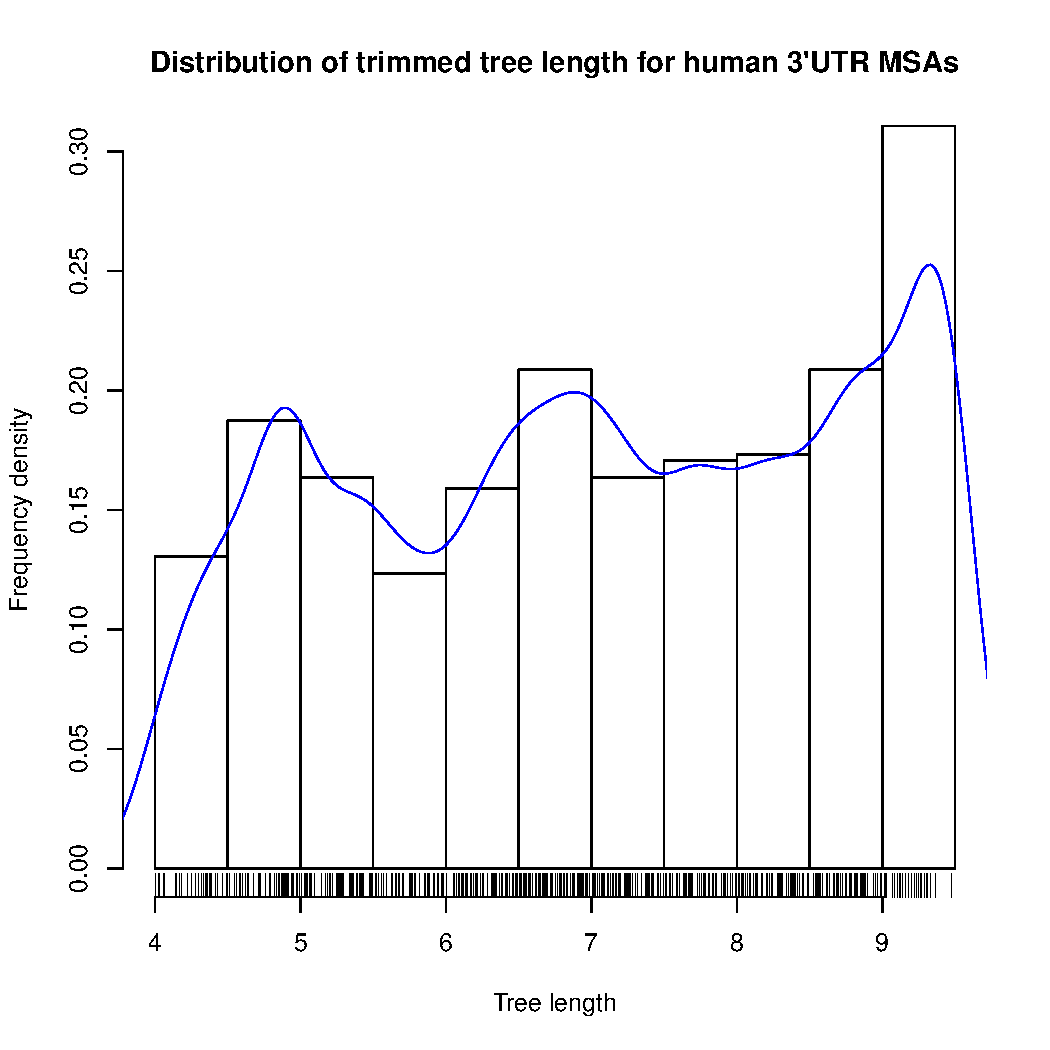
\includegraphics[width = \textwidth]{DistTrimTreeLen}
    \caption[Distribution of trimmed tree length for human 3'UTR MSAs]{\label{human3UTRtrimtreeLenDist}Distribution of trimmed tree length for human 3'UTR MSAs. The figure is similar to that Figure~\ref{human3UTRtreeLenDist}. However, MSAs are trimmed according to the new tree and those with total tree length beyond 4 to 10 region are removed.}
  \end{center}
\end{figure}

\FloatBarrier

As a contrast, if we trim the tree in a conserved manner, we would get good alignment but bad variation. For example, like said in Figure~\ref{Hg18Simi44way}, if we remove those species with less than 10\% coverage, we get a 33way tree with length 6.463.

\FloatBarrier
\begin{figure}[!hbp]
  \begin{center}
    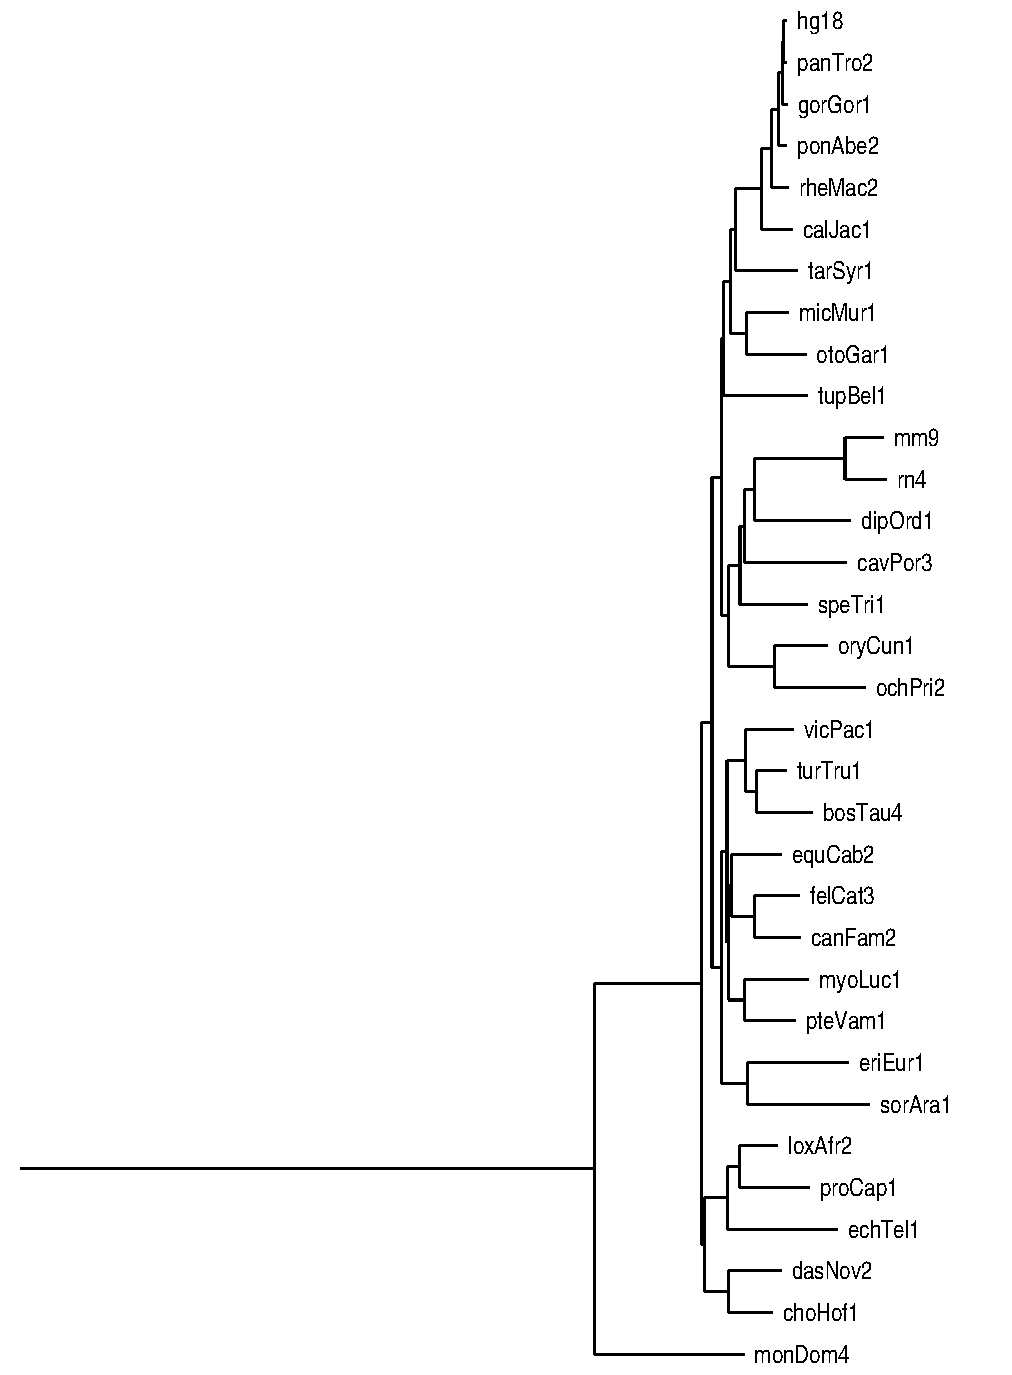
\includegraphics[height = 0.95\textheight]{33way-eps-converted-to}
    \caption[Hg18 33way alignment: trimmed tree]{\label{tree33way} Hg18 33way alignment: trimmed tree. This tree is built from the 44way tree from UCSC with removing low coverage species.}
  \end{center}
\end{figure}
\FloatBarrier


Since the final goal is on RNA-secondary structure level,  probably we need criteria other than conservation and gappiness which obviously bias to conserved alignments, such as Mutual Information or Transat scores or those methods mentioned at the beginning of this section (mlocarna and simulfold).





\subsection{Incoperating the RIP-Chip enrichment data}
Briefly, the in vivo RIP-Chip data from \cite{Hogan2008} have been collected for all the proteins (human, yeast and fly) on Table~\ref{RBPs}, so that for most of the transcripts we now have their enrichment values in the copurifying experiments with proteins. These transcripts  are then classified into "bound", "unbound" and "unsure" sets using similar approach as \cite{Li01062010} did. 

Computing the accessibilities based on "bound" and "unbound" sets are much more reasonable than simply considering the matched motif sequence hits. This is because of the obvious fact that sequence matching has a very high false positive rate for protein binding motifs though the proteins are known to be sequence-specific binding. We could further compare the difference between false positive matchings and true positive matchings, which would potentially improve binding motif discovery.

By far, I have performed a pilot study on Msl5 and Khd1 proteins in yeast using "bound" set and observed significant difference (p-values smaller than 0.05) on accessibilities between motif hits and the whole 3'UTR (background) region; also for "unbound" set there is no significant difference. However, I still need to test this for all the other proteins before any conclusion could be drawn. Also, the results are based on raw alignment from UCSC without realignment. The alignments may need to be tuned and the results may differ.  





\bibliography{results}
\bibliographystyle{unsrt}



\end{document}
\endinput
%%
%% End of file `ubcsample.tex'.

